
\documentclass[12pt,a4paper]{book}		
%Book style with A4 paper, chapeters start on left page only, using times fonts

\usepackage[T1]{fontenc}
\usepackage{ae,aecompl}
\usepackage{times}
% Selects font encoding
\usepackage{rotating}

\usepackage{subcaption}

\usepackage{caption}
\usepackage{float}

\usepackage{geometry}
\geometry{b5paper}

\usepackage{pgfplots}

\usepackage{pdfpages}

\usepackage{longtable}
\usepackage{supertabular}
\usepackage{cleveref}
\usepackage{lscape}

\usepackage{array}
\usepackage{calc}

\usepackage{natbib}								% Correct citations


\usepackage{url}
% breakes long urls prettier over more than one line

\usepackage[colorlinks=true,pageanchor=true,linkcolor=black,anchorcolor=black,filecolor=black,citecolor=black,menucolor=black,pagecolor=black,urlcolor=black,bookmarksopen=true,bookmarksopenlevel=1]{hyperref}
% Creates hyperlinks of references/urls. Default color is blue but the settings above change the colors to black.

\usepackage{parskip}
% Starts new paragraphs without indentation but with some space between the new and the previous paragraph.

\usepackage{multirow}
% Used to create tables with rows/cols spanning over se

\usepackage{graphicx}
% Used to include images with the includegraphics command

\usepackage{pdfpages}
% Used to import pages from or whole pdf-documents

\usepackage{amsmath}
% Used for math symbols
\usepackage{amssymb}


% Used for abbriviations
\usepackage{nomencl}
\renewcommand{\nomname}{Abbreviations}
\renewcommand{\nomlabel}[1]{\textbf{#1}} % make abbreviations bold
\makenomenclature
\newcommand*{\nom}[2]{#1\nomenclature{#1}{#2}}
\cleardoublepage

%\usepackage{makeidx}
%\makeindex
% Needed to create glossaries


% \usepackage[number=none]{glossary}
% \makeglossary
% To create glossary and list of acronyms. Other packages may also be used. Page numbering is turned off in the final list.

% Creates a new glossary for abbreviations
% \newglossarytype[abr]{abbr}{abt}{abl}

% \newglossarytype[alg]{acronyms}{acr}{acn}
%\newcommand{\abbrname}{Abbreviations} 
%\newcommand{\shortabbrname}{Abbreviations}
%\makeabbr

% Creates a new command for argmax with underset
\newcommand{\argmax}[1]{\underset{#1}{\operatorname{arg}\,\operatorname{max}}\;}




% The below code sets the margins of the document.
% See: http://web.image.ufl.edu/help/latex/margins.shtml for an explanation of the margins.

%\oddsidemargin 5mm
%\evensidemargin 5mm
%\textwidth 150mm
%\topmargin 0mm
%\headheight 0mm
%\textheight 225mm
%\footheight 0mm



% Hyphens
\hyphenation{Sem-Eval Senti-Map Senti-Graph Senti-Stack Java-Script hand-ling domene-uavhengig Timeline-Stats Tweet-Count}

% Contents 
\setcounter{secnumdepth}{3}
% \setcounter{tocdepth}{3}

\usepackage{color}
% To give color to the text. It is only used to highlight the instructions in this document and it can be removed.


\def\thesisTitle{Your Thesis Title} 
% Defines the title of the thesis.

\def\thesisAuthor{Mikael Brevik \&  {\O}yvind Selmer} 
% Defines the name of the author (that is your name).



\begin{document}

% Information pages about your thesis
\begin{titlepage}
\begin{center}

\vspace*{2cm}

\huge{\textcolor{blue}{\thesisTitle}}


\vspace{.5cm}
\large{\textcolor{blue}{\thesisAuthor}}



\vspace{1cm}


\vspace{1cm}
\huge{Master's Thesis}


\vspace{6cm}


\end{center}
\normalsize

\begin{table}[!h]
\begin{tabular}{ll}
\multirow{4}{*}{
\includegraphics[width=20mm]{../img/logo}} & \\
& Department of Computer and Information Science \\
& Faculty of Information Technology, Mathematics and Electrical Engineering \\
& Norwegian University of Science and Technology \\

\end{tabular}
\end{table}



\vspace{.5cm}


\begin{center}
\today
\end{center}

\end{titlepage}

\clearpage

\thispagestyle{empty}

\vspace*{15cm}

\textcolor{red}{(This page will also be removed by NTNU-trykk and replaced with a template. This page is known as the colophon page, or kolofon side)}

\textcolor{red}{You will need the two ISBN numbers and the internal NTNU ''thesis number'' that year. All this can be 
obtained from  \url{http://ojapp01.itea.ntnu.no:7780/isbnprovider/start.do}} 

\textcolor{red}{The ISSN serial number is the same for all doctoral theses at NTNU, and is 1503-8181.}
\clearpage





\pagestyle{plain}
% Includes page number at the bottom of the page.
\pagenumbering{roman} 				
% Uses small roman numbers for page numbering.
\setcounter{page}{1}
% Resets the page counter to 1.

% The start of the actual thesis.
\section*{Abstract}
\addcontentsline{toc}{chapter}{Abstract}

The social micro-blog site Twitter grows in user base each day and has become an attractive platform for companies, politicians, marketeers, and others wishing to share information and/or opinions. With a growing user market for Twitter, more and more systems and research are released for taking advantage of its informal nature and doing opinion mining and sentiment analysis. 

This master thesis describes a system for doing Sentiment Analysis on Twitter data and experiments with grid searches on various combinations of machine learning algorithms, features and preprocessing methods to achieve so. The classification system is fairly domain independent and performs better than baseline. 

This system is designed to be fast enough to classify big amounts of data and tweets in a stream, and provides an application program interface (API) to easily transfer data to applications or end users. 

Three visualisation applications are implemented, showing how to use the API and providing examples of how sentiment data can be used.

The main contributions are: 

\begin{itemize}
\item[\textbf{C1}] A literary study of the state-of-the-art for Twitter Sentiment Analysis.

\item[\textbf{C2}] The implementation of a general system architecture for doing Twitter Sentiment Analysis. 

\item[\textbf{C3}] A comparison of different machine learning algorithms for the task of identifying sentiments in short messages in a fairly semi-independent domain.

\item[\textbf{C4}] Implementations of a set of visualisation applications, showing how to use data from the generic system and providing examples of how to present sentiment analysis data.
\end{itemize}

\clearpage

\section*{Sammendrag}

Den sosiale mikrobloggingsnettstedet Twitter er i kontinuerlig vekst og har blitt et attraktivt verkt\o y for bedrifter, politikere, markedsf\o rere og andre som \o nsker \aa~dele informasjon og/eller meninger. Med \o kende brukermasse, kommer det ut flere og flere systemer og forskningsresultater relatert til Twitter, sentimentanalyse og meningsm\aa linger.

Denne masteroppgaven definerer et system for \aa~utf\o re sentimentanalyse p\aa~data fra Twitter og oppn\aa r dette ved \aa~eksperimentere med parameters\o k p\aa~forskjellige kombinasjoner av maskinl\ae ringsalgoritmer, funksjoner og preprosesseringsmetoder. Det utviklede systemet er forholdsvis domene-uavhengig og har bedre ytelse enn baseline.

Dette systemet ble designet for \aa~takle store mengder data og klassifisere tweets i datastr\o mmer. For {\aa} enkelt tilby data til sluttbrukeren, ble et "application program interface"~(API) definert.

Et sett med visualiseringsapplikasjoner ble implementert for {\aa} vise bruken av API-et og hvordan sentiment data kan bli brukt og presentert.

Hovedbidragene fra oppgaven er f\o lgende:

\begin{itemize}
\item[\textbf{C1}] Oppgaven definerer en state-of-the-art for Twitter Sentimentanalyse (TSA).

\item[\textbf{C2}] Et generelt systemarkitektur for TSA ble utviklet og implementert.

\item[\textbf{C3}] Forskjellige maskinl\ae ringsalgoritmer er satt i mot hverandre for \aa~ best finne sentiment i korte meldinger p\aa~en relativt domeneuavhengig m{\aa}te.

\item[\textbf{C4}] Visualiseringsapplikasjoner er implementert, og viser hvordan en kan bruke dataen fra det generelle systemet og hvordan sentimenter kan bli presentert og brukt.
\end{itemize}

\clearpage
\section*{Preface}
\addcontentsline{toc}{chapter}{Preface}

This thesis is submitted to the Norwegian University of Science and Technology (NTNU) for partial fulfilment of the requirements for the Master's degree.

This Master's Thesis work has been performed at the Department of Computer and Information Science, NTNU, Trondheim, with Bj\"{o}rn Gamb\"{a}ck and with co-supervisor Lars Bungum.



\cleardoublepage
\section*{Acknowledgements}
\addcontentsline{toc}{chapter}{Acknowledgements}

We would like to thank our supervisor Bj\"{o}rn Gamb\"{a}ck and co-supervisor Lars Bungum, for invaluable response and guidance for this project and to Amitava Das for inital discussions regarding sentiment analysis and guidance during the pre-project.

We would also like to thank the organizers of SemEval'13 for the data sets used to train our system, in addition to our own little data set. 

A big thanks to the human annotators, volunteering to help us generate a data set of our own.  

\cleardoublepage

\tableofcontents
% Prints the table of contents							
\addcontentsline{toc}{chapter}{Contents}
\clearpage

\listoftables					
% Prints a list of your tables. Remember to use caption on the tables.
\addcontentsline{toc}{chapter}{List of Tables}
\clearpage

\listoffigures									
% Prints a list of your figures. Remember to use caption on the figures.
\addcontentsline{toc}{chapter}{List of Figures}
\cleardoublepage


% Prints a list of abbreviations
\addcontentsline{toc}{chapter}{Abbreviation}
% \printabbr


\cleardoublepage


\pagenumbering{arabic} 				
% Uses arabic numbers (normal numbers) for page numbering.
\setcounter{page}{1}
% Resets the page counter to 1.


% The chapters
\chapter{Introduction}

The introduction chapter first defines the task description. Background and Motivation for this task is given in~section~\ref{sec:motivation}, followed by an overview of the project goals in~section~\ref{sec:projectgoals} and in~section~\ref{sec:contribution} the project contribution is summarised. In the last section of the introduction, an overview of this report is described. 

This report is the result of a Master thesis at Department of Computer and Information Science, \nom{NTNU}{Norwegian University of Science and Technology}, 2013. 

\section{Task Description}
\label{sec:task}

The task was given by Bj\"{o}rn Gamb\"{a}ck and Lars Bungum at IDI, NTNU

\begin{center} \Large Sentiment Analysis using the Twitter Corpus \end{center}
\begin{quotation}
In recent years, micro-blogging has become prevalent, and the Twitter API allows users to collect a corpus from their micro-blogosphere. The posts, named tweets are limited to 140 characters, and are often used to express positive or negative emotions to a person or product.

In this project, the goal is to use the Twitter corpus to do Sentiment Analysis and develop tools for visualising the results. Pak and Paroubek (2010) have shown how to do this using frameworks like Support Vector Machines (SVMs) and Conditional Random Fields (CRFs), benchmarked with a Naive Bayes Classifier baseline. They were unable to beat the baseline, and the goal of this project will be to experiment with these and other machine learning frameworks as Maximum Entropy learners to try to beat the baseline.
\end{quotation}


\section{Background and Motivation}
\label{sec:motivation}

Twitter has become a popular social media service often referred to as a micro-blogging site. On Twitter users can post messages of maximum 140 characters, called tweets, on their own \emph{timeline}. A timeline is a collection of all user submitted tweets and all tweets from the other users that a user is connected to (following). Tweets can be categorized by using hashtags. A hashtag can, for instance, look like \emph{\#happy} or \emph{\#obama2012}. By annotating the tweets with this tag, users can find similar tweets across Twitter. Tweets often also contain references to other users by using the $@$-character followed by the user name (e.g. \emph{$@$obama}) or references to pictures or articles via URLs.

Twitter has grown very rapidly and the usage statistics is ever changing. In June 2012, there were posted over 400 million tweets every day~\citep{site:twitterusage}. With over 500 million users, where about 170 million of these are active ones~\citep{site:users}, it is safe to say that Twitter offers a lot of data.

The informal nature of Twitter leads to a lot of sentiments being posted and this has led Twitter to being a gold mine for sentiment analysis (\nom{SA}{Sentiment Analysis}). Many systems have used Twitter as corpus for SA. The first one to really use Twitter as a corpus was Sentiment140 (previously known as TwitterSentiment) by a group of Stanford students~\citep{article:go}. After this paper, and as Twitter grew in popularity, many other systems have been developed. Some of the later ones are TwiSent and C-Feel-IT~\citep{mukherjee2012twisent}, Tweenator~\citep{saif2012semantic} and MSAS~\citep{chamlertwat2012discovering}.

Many system uses a single step, three way, classification for sentiments. But another approach is to do a two step classification, where firstly the subjectivity is classified and in step two, the polarity. Subjectivity classification is the task of classifying if a tweet is subjective or objective. \cite{article:pak} counted word frequencies in a subjective vs an objective set of tweets; the results showed that interjections and personal pronouns are the strongest indicators of subjectivity. If the tweet is classified as objective (or neutral), no further classification is required. If the tweet is subjective, however, it requires polarity classification. Polarity classification will classify between positive and negative tweets.~\cite{article:omg} experimented with different solutions for tweet polarity classification, and found that the best performance came from using n-grams together with lexicon and micro-blog features. Interestingly, performance dropped when a part-of-speech (POS) tagger was included. They speculate that this can be due to the accuracy of the POS tagger itself, or that POS tagging just is less effective for analysing tweet polarity.

The growth in Twitter users and status updates (tweets) over the last years has made Twitter an attractive platform for companies, marketeers, politicians and others who are looking for feedback. Manually collecting information like this is a tedious if not impossible task.

The informal texts on social media represent challenges for traditional natural language processing systems. These texts are short, and often con- tain misspellings, slang and abbreviations. The challenge of handling such a vocabulary has only been researched over the last few years.

Another interesting feature is that Twitter messages offer a lot of meta data and information about their origin, such as location, language, and more. These data could for example be used to filter out and classify tweets from a certain event, like a festival or a conference.

For visualising sentiment data, not as much has been done. Sentiment140, by~\cite{article:gimpel}, has some rudimentary visualising with pie and bar charts\footnote{\url{http://www.sentiment140.com/}}. \cite{article:wefeelfine} developed an emotional search engine with different advanced techniques for visualising mood, but not for three way classification for sentiment on Twitter.

\section{Project Goals}
\label{sec:projectgoals}

In this section, the main goals of for this project are described.

\begin{description}

\item[G1] \textbf{Experiment with different models for doing sentiment analysis} \\
	Design and implement different models for doing sentiment analysis. Experiment with these models and find the model with highest accuracy and beating the baseline the most. 
	
\item[G2] \textbf{Develop tools for visualising sentiment classified tweets} \\
    Data is wasted if it is not used for anything. Data needs proper, usable, summarising and visualisation tools to be of use. One of the goals of this project is to come up with, plan and develop tools that are useful for showing the real value of sentiment classified tweets. To be able to make visualisation applications, we also need a way to distribute the data through a documented interface. 

\end{description}

\section{Contributions}
\label{sec:contribution}

\begin{itemize}
\item[\textbf{C1}] This thesis provides a definition of the state-of-the-art for Twitter Sentiment Analysis.

\item[\textbf{C2}] A general system architecture for doing Twitter Sentiment Analysis is implemented. 

\item[\textbf{C3}] Different machine learning algorithms are compared for the task of identifying sentiments in short messages in a fairly semi-independent domain.

\item[\textbf{C4}] Visualisation applications are implemented, showing how to use data from the generic system and examples of how to show sentiment analysis data.
 
\end{itemize}

\section{SemEval'13}

During the course of this project, a workshop for doing semantic analysis systems was being held, called SemEval'13. The workshop had several different shared tasks, amongst others a task for building a message polarity classification system. In relation to this workshop, data sets were published to the participants. To take advantage of this and to formally test our system, we participated in the workshop and submitted a paper. 

\section{Thesis Structure}
\label{sec:structure}

In Chapter 2, the existing solutions and current state of the art is described. In Chapter 3, data sets and machine learning theory is described. The system architecture and model is presented and documented in Chapter 4. Chapter 4 also has a complete description of the visualisation application architecture and how the applications work. In Chapter 5 experiments and results regarding different approaches for doing Sentiment Analysis is described. Chapter 6 includes evaluation and discussions of the results. In Chapter 7 the report is concluded and future work is described. 

% \section{Examples REMOVEME!}

% This is an example of a reference \cite{copland2000}.

%  This is a reference to Table \ref{tab:1-relations} and to Figure \ref{fig:1-studies_contributions_papers}.

% A glossary example which will be included in the glossary at the end of the document:
% \glossary{name=Newton,description=Unit of force but may also refer to Sir Isaac Newton.}

% An abbrevation example which will be included in the list of abbrevations: 
% \abbr{name=NTNU,description=Norwegian University of Science and Technology}

% To use the glossary:
% 1. Compile the latex document.
% 2. Run the makeGlossary.{bat|sh} (.bat for windows, .sh for Linux/Unix). This script ASSUMES that your latex file is
% called document.tex 
% 3. Compile the latex document again (I have sometimes experienced some error messages but as long as I compile a
% couple of times it is ok)

\chapter{State of the Art}

A systematic literature review (\nom{SLR}{Systematic Literature Review}) was conducted to establish the state of the art of a Twitter Sentiment Analysis (\nom{TSA}{Twitter Sentiment Analysis}) system. The method and results is documented in this chapter. The first section, Section~\ref{sec:slrintro}, covers the introduction and defines our research questions. The review method is described in Section~\ref{sec:slrmethod} and the result in Section~\ref{sec:slrresults}.

\section{Introduction}
\label{sec:slrintro}

SLRs are still new in the field of computer science. There are few examples of an SLR in practice. The method we used is heavily inspired by the documentation paper by~\cite{paper:slrdesc} and the Master's thesis by~\cite{master:slr}. \\

\noindent We defined our research questions (\nom{RQ}{Research Question}) as the following:

\begin{description}

\item[RQ1] What are some of the existing solutions for SA (sentiment analysis) in the Twitter Corpus.
\item[RQ2] How does the different solutions found by addressing RQ1 compare to each other with respect to micro-blogs like Twitter.
\item[RQ3] What is the strength of the evidence in support of the different solutions?
\item[RQ4] What implications will these findings have when creating the application/system?

\end{description}

\section{Review method}
\label{sec:slrmethod}

In this section we will describe our process step by step according to the systematic literature review. 

\subsection{Planning}

\begin{description}

	\item[1. Identification of the need for a review] \hfill \\
		Assumed that a review is needed for this project. 
		
	\item[2. Commissioning a review] \hfill \\
		Assumed to be commissioned for this project, so no commission report was produced. 

	\item[3. Specifying the research question(s)] \hfill \\
		We defined the RQs based on what we felt needed to be researched when finding the state-of-the-art for sentiment analysis systems on Twitter. The RQs can be seen in Section~\ref{sec:slrintro}. 

	\item[4. Developing a review protocol] \hfill \\
		The review protocol \nom{SLRP}{Systematic Literature Review Protocol} was developed in the early stages of the project. After the first revision it was evaluated by the project supervisor. The protocol was revised several times during the execution of the review.
	

	\item[5. Evaluating the review protocol] \hfill \\
		The protocol was evaluated by the project supervisor. 

\end{description}


\subsection{Conducting}

\begin{description}

	\item[1. Identification of research] \hfill \\
		We defined a series of keywords and synonyms to construct a search string to use. The search string was defined to find papers relevant to our research questions. The development of this search string is documented by Appendix~\ref{apx:slrp}. The search string we used was:
		
		\begin{verbatim}
		("Sentiment Analysis" OR "Sentiment Classification" 
		OR "Opinion Mining") AND (Twitter OR Microblog)
		\end{verbatim}
		
		For the search domain, we used Google Scholar. Google Scholar accumulates results from several different sources and gave many results for our search. A lot of the results given corresponded to the studies handed out by the project supervisor, a domain expert. 
		
		We limited the search to only give papers released after 2008. This is due to Twitter being as new as it is.
		
		The search resulted in 1060 papers, but after the first 8 pages of results (with 10 papers per page), we found that the papers were mostly irrelevant and we had limited resources and time for handling all 1060 papers. This resulted in a set of 80 papers, ready to go through the selection process.
		
		

	\item[2. Selection of primary studies] \hfill \\
		First, we defined a set of primary inclusion criteria. These criteria were applied to the title and abstract of the study. If a paper did not pass the criteria, it was dropped from the set. Secondly we defined secondary inclusion criteria. These criteria were checked against the full text of the study. These inclusion criteria are documented in the protocol in~\autoref{apx:slrp}. 
		
		After both selection processes, we had a set of 23 papers. 

	\item[3. Study quality assessment] \hfill \\
		With the help of \cite{paper:slrdesc} we defined a set of 10 quality criteria. All of the criteria are documented in the protocol in~\autoref{apx:slrp}. Each of the papers in our set was assessed with all of these criteria. If the paper met the criteria, it would get 1 point, if met partly it would get 0,5 points, and if it did not meet the criteria it would get 0 points. 
		
		The papers with the lowest score did not get taken as much into consideration when defining the state-of-the-art. 
		
	\item[4. Data extraction and monitoring] \hfill \\
		We defined a set of fields and information categories we thought were important in order to answer our research questions. These data features were used to generate a table of information. The information was retrieved by reading the papers and manually extracting the data we needed.
	

	\item[5. Data synthesis] \hfill \\
		This step was included in the data extraction step.
\end{description}

% This probably shouldn't be here but in the SLR chapter..
% For this report, the data synthesis is included as a part of the data extraction. 

\subsection{Reporting}


\begin{description}

	\item[1. Specifying dissemination strategy] \hfill \\
		As this is for a master thesis, the result of the SLR is presented in this report.  

	\item[2. Formatting the main report] \hfill \\
		The SLR was written as a section in this project report. 

	\item[3. Evaluating the report] \hfill \\
		It is mandatory for an expert to review this report as well as a project supervisor, as it is a report for a master thesis.

\end{description}

\section{Results}
\label{sec:slrresults}

In this section the result of the systematic literature review is presented. In Section~\ref{sec:selected} all of the extracted data from the selected studies are presented. The assessed quality of the articles is also documented here.

Section~\ref{sec:stateofart} answers the research questions given as a part of the SLRP. 

\subsection{Selected studies} 
\label{sec:selected}

In this section all of the selected studies are presented in table format as a part of the data extraction step in the SLR. The results can be found in~\autoref{tab:extraction}. In addition to the data features defined in the review protocol, the total quality is added to be a part of the extraction table.


\begin{sidewaystable}
    \centering
    \caption{Data extraction step, table 1/4. Showing data as per defined in the SLRP in attachment \autoref{apx:slrp}}
    \scriptsize
    \label{tab:extraction}
    \begin{longtable}{|c|p{3cm}|p{4cm}|p{0.6cm}|p{1cm}|p{1.3cm}|p{4cm}|p{3cm}|p{0.3cm}|} 
    
    \hline
    \textbf{\#ID} & \textbf{Authors} & \textbf{Title} & \textbf{Pub. Year} & \textbf{System name} & \textbf{ML Algorithm} & \textbf{Dataset} & \textbf{Findings} \& \textbf{Conclusions} & \textbf{QA} \\ 
    \hline
    
    S1 & Hassan Saif, Yulan He \& Harith Alani & Semantic Smoothing for Twitter Sentiment Analysis & 2012 & - & NB & http://twittersentiment.appspot.com/ & Slight improvement by .3\% & 7,5 \\ \hline  
    
    S2 & Subhabrata Mukherjee, Akshat Malu, A.R. Balamurali, Pushpak Bhattacharyya & TwiSent: A Multistage System for Analyzing Sentiment in Twitter & 2012 & TwiSent & NB & C-Feel-IT dataset.  & Improvements with filtering/ normalization. Best: 66,69\% with manually annotated dataset  & 8,5 \\ \hline  
    
    S3 & Adam Bermingham \& Alan Smeaton & Classifying Sentiment in Microblogs:Is Brevity an Advantage? & 2010 & - & NB, SVM & "CLARITY dataset (removed due to Twitter terms), Pang \& Lee's movie corpus,TREC Blogs06 corpus and a collection of microreviews from Blippr" & Accuracy of 74.85\% using NBC and unigrams. Easier to classify microblogs than long texts  & 9,0 \\ \hline  
    
    S4 & Wilas Chamlertwat, Pattarasinee Bhattarakosol, Tippakorn Rungkasiri, Choochart Haruechaiyasak & Discovering Consumer Insight from Twitter via Sentiment Analysis & 2012 & MSAS & SVM, Lexical (non ML) & Self compiled, manually annotated 600 tweets & Sentiment Analysis can be useful for consumer research. No accuracy for classification.  & 8,0 \\ \hline  
    
    S5 & Dmitry Davidov, Oren Tsur \& Ari Rappoport & Enhanced Sentiment Learning Using Twitter Hashtags and Smileys & 2010 & - & HFW/CW & Dataset by Brendan O?Connor. Hashtags and smileys as training labels. & Hashtags and smilies works good for SA  & 6,5 \\ \hline  
    
    S6 & Murphy Choy, Michelle L.F. Cheong, Ma Nang Laik \& Koo Ping Shung & "A sentiment analysis of Singapore Presidential Election 2011 using Twitter data with census correction" & 2011 &  &  &  & "Given proper recalibration using census information, the twitter information can translate into pretty accurate information about the political landscape."  & 5,5 \\ \hline  
    
    S7 & Hassan Saif, Yulan He \& Harith Alani & Semantic Sentiment Analysis of Twitter & 2012 & Tweentor & NB & Stanford Twitter Sentiment Corpus, Health Care Reform, Obama-McCain Debate & Improvements by using semantic features on wide range topics. Acc: 83.9\%  & 9,0 \\ \hline  
    
    
    \end{longtable}
\end{sidewaystable}

\begin{sidewaystable}
    \centering
	\caption{Data extraction step, table 2/4. Showing data as per defined in the SLRP in attachment \autoref{apx:slrp}}
    \scriptsize
    \begin{longtable}{|c|p{3cm}|p{4cm}|p{0.6cm}|p{1cm}|p{1.3cm}|p{4cm}|p{3cm}|p{0.3cm}|} 
    
    \hline
    \textbf{\#ID} & \textbf{Authors} & \textbf{Title} & \textbf{Pub. Year} & \textbf{System name} & \textbf{ML Algorithm} & \textbf{Dataset} & \textbf{Findings} \& \textbf{Conclusions} & \textbf{QA} \\ 
    \hline
    
    S9 & Lei Zhang, Riddhiman Ghosh, Mohamed Dekhil, Meichun Hsu \& Bing Liu & "Combining Lexicon-based and Learning-based Methods for Twitter Sentiment Analysis" & 2011 &  & SVM, Lexical &  & Outperforms approaches that use lexical or supervised methods alone  & 8,5 \\ \hline  
    
    
    S11 & Alec Go, Lei Huang, Richa Bhayani & Twitter Sentiment Analysis & 2009 & Sentiment140 & NB, SVM & http://www.stanford.edu/~alecmgo/cs224n/ twitterdata.2009.05.25.c.zip & ~85\% - bias accuracy.  & 9,0  \\ \hline  
    
    S12 & James Spencer \& Gulden Uchyigit & Sentimentor: Sentiment Analysis of Twitter Data & 2012 & Sentimentor & NB &  & 52\% for three classes(pos,neg and objective) using bigrams without POS tagging  & 7,5 \\ \hline  
    
    S13 & Amir Asiaee T, Arindam Banerjee, Mariano Tepper \& Guillermo Sapiro  & If You are Happy and You Know It... Tweet & 2012 &  & NB,SVM,k-NN, DL &  & 82.95\% accuracy with NB on tweets about the weather  & 8,5 \\ \hline  
    
    S14 & Finn Arup Nielsen & "A new ANEW: Evaluation of a word list for sentiment analysis in microblogs" & 2011 &  & Lexical & Labeled language data created with Amazon Mechanical Turk(AMT) & The AFINN word list performs slightly better than ANEW in Twitter sentiment analysis  & 7,5 \\ \hline  
    
    S15 & Luciano Barbosa \& Junlan Feng & Robust sentiment detection on Twitter from biased and noisy data & 2010 & TwitterSA & SVM & Used Twendz, Twitter Sentiment and TweetFeel to collect data & By using data with noisy labels as input, they achieved a more abstract representation of Twitter messages than raw words.  & 8,5 \\ \hline  
    
    \end{longtable}
\end{sidewaystable}

\begin{sidewaystable}
    \centering
	\caption{Data extraction step, table 3/4. Showing data as per defined in the SLRP in attachment \autoref{apx:slrp}}
    \scriptsize
    \begin{longtable}{|c|p{2.5cm}|p{4cm}|p{0.6cm}|p{1cm}|p{1.3cm}|p{4cm}|p{3cm}|p{0.3cm}|} 
        
    \hline
    \textbf{\#ID} & \textbf{Authors} & \textbf{Title} & \textbf{Pub. Year} & \textbf{System name} & \textbf{ML Algorithm} & \textbf{Dataset} & \textbf{Findings} \& \textbf{Conclusions} & \textbf{QA} \\ 
    \hline

    
    S16 & Younggue Bae \& Hongchul Lee & "A Sentiment Analysis of Audiences on Twitter: Who Is the Positive or Negative Audience of Popular Twitterers? " & 2011 &  & Used LIWC2007 dictionary to extract sentiment & Collected tweets from celebrities and their mentions & & 5,5  \\ \hline  
    
    S17 & Mauro Cohen, Pablo Damiani, Sebastian Durandeu, Renzo Navas, Hern\'{a}n Merlino, Enrique Fern\'{a}ndez & Sentiment Analysis in Microblogging: A Practical Implementation & 2011 & - & NB & Manually gathered and annotated. 1500 tweets & Not as good accuracy as previous systems & 4,0 \\ \hline  
    
    S18 & Roberto Gonz\'{a}lez-Ib\'{a}\~{n}ez, Smaranda Muresan, Nina Wacholder & Identifying Sarcasm in Twitter: A Closer Look & 2011 & - & SMO, LogR & Data collected by using hashtag search. 900 tweets & Best result (75.89\%) was achieved in the polarity- based classification P-N. Automatic classification can be as good as human classification; however, the accuracy is still low & 9,5 \\ \hline  
    
    S19 & Akshi Kuma, Teeja Mary Sebastian & Sentiment Analysis on Twitter & 2012 & - & None. POS and own alg. &  & "The initial results show that it is a motivating technique." No stated accuracy & 7,5 \\ \hline  
    
    S20 & Alexander Pak, Patrick Paroubek & Twitter as a Corpus for Sentiment Analysis and Opinion Mining & 2010 & - & NB & http://www.stanford.edu/ ~alecmgo/cs224n/ twitterdata.2009.05.25.c.zip & ~63\% accuracy using bigrams and POS tagging & 10 \\ \hline  
    

    
    
    \end{longtable}
\end{sidewaystable}

\begin{sidewaystable}
    \centering
	\caption{Data extraction step, table 4/4. Showing data as per defined in the SLRP in attachment \autoref{apx:slrp}}
    \scriptsize
    \begin{longtable}{|c|p{3cm}|p{4cm}|p{0.6cm}|p{1cm}|p{1.3cm}|p{4cm}|p{3cm}|p{0.3cm}|} 
    
    \hline
    \textbf{\#ID} & \textbf{Authors} & \textbf{Title} & \textbf{Pub. Year} & \textbf{System name} & \textbf{ML Algorithm} & \textbf{Dataset} & \textbf{Findings} \& \textbf{Conclusions} & \textbf{QA} \\ 
    \hline
    
    S21 & Long Jiang, Mo Yu, Ming Zhou, Xiaohua Liu, Tiejun Zhao & Target-dependent Twitter Sentiment Classification & 2011 & - & SVM & "Subjectivity: Manually annotated 727 tweets for each class. Polarity: Manually annotated 268 tweets for each (pos, neg)" & "Subjectivity: 85.6\%. Polarity: 68.2\%" & 8,5 \\ \hline  
    
    S22 & Kun-Lin Liu, Wu-Jun Li \& Minyi Guo & Emoticon Smoothed Language Models for Twitter Sentiment Analysis & 2012 & ESLAM & Unigram, MLE & Sanders Corpus (5513 manually labeled tweets with one of the four different topics: Apple, Google, Microsoft, and Twitter) & ESLAM performs better than both emoteicons(distant supervised) and manually annotated tweets(fully supervised) alone & 10 \\ \hline  
    

    
    S23 & Efthymios Kouloumpis, Theresa Wilson, Johanna Moore & Twitter Sentiment Analysis: The Good the Bad and the OMG! & 2011 & - & AdaBoost.MH & Gathered by hash, http://twittersentiment.blogspot.com and iSieve Corporation for evaluating data & Hash + Emoticons result in 75\% accuracy & 8,0 \\ \hline  
    
    S25 & Apoorv Agarwal, Boyi Xie, Ilia Vovsha, Owen Rambow, Rebecca Passonneau & Sentiment Analysis of Twitter Data & 2011 & - & SVM & "Data by NextGen Invent (NGI). Manually annotated 11,875 tweets, non-bias tweets" & A gain of 4\% on unigram 3-way classification. Acc: 60.83\% & 10 \\ \hline  
    
    S26 & Asli Celikyilmaz, Dilek Hakkani-T\"{u}r \& Junlan Feng  & Probabilistic Model-based Sentiment Analysis Of Twitter Messages & 2010 &  & Used LDA to extract a polarity lexicon & Collected 2 million tweets using Twitter search API from September 2009 to June 2010. Keywords related to mobile operation. Made two manually annotated subsets from this collection. & Relatively 10\% better F-measure with unigrams than baseline for classification with text normalization and all word unigram, bigram and trigrams as features. & 7,5 \\ \hline  
    
    \end{longtable}
\end{sidewaystable}


In \autoref{tab:quality} all the individual points for the quality criteria are presented. The criteria are defined as a part of the review protocol. The average criterion score was 8.0.

\begin{table}
    \centering
    \scriptsize
    
    \setlength\tabcolsep{2pt}
    \def\arraystretch{1.4}%  1 is the default, change whatever you need
    \begin{tabular}{|c|c|c|c|c|c|c|c|c|c|c||c|} 
    
    \hline
    \textbf{\#ID} & \textbf{QC1} & \textbf{QC2} & \textbf{QC3} & \textbf{QC4} & \textbf{QC5} & \textbf{QC6} & \textbf{QC7} & \textbf{QC8} & \textbf{QC9} & \textbf{QC10} & \textbf{Total} \\
    \hline
    
    \textbf{S1} & 1.0 & 0.5 & 1.0 & 0.5 & 1.0 & 1.0 & 0.5 & 0.5 & 0.5 & 1.0 & 7.5 \\ \hline
    \textbf{S2} & 1.0 & 1.0 & 1.0 & 0.5 & 1.0 & 1.0 & 1.0 & 0.5 & 0.5 & 1.0 & 8.5 \\ \hline
    \textbf{S3} & 1.0 & 1.0 & 0.5 & 0.5 & 1.0 & 1.0 & 1.0 & 1.0 & 1.0 & 1.0 & 9.0 \\ \hline
    \textbf{S4} & 1.0 & 1.0 & 0.5 & 0.5 & 1.0 & 1.0 & 1.0 & 0.5 & 0.5 & 1.0 & 8.0 \\ \hline
    \textbf{S5} & 1.0 & 0.5 & 0.5 & 0.5 & 1.0 & 1.0 & 0.0 & 0.5 & 1.0 & 0.5 & 6.5 \\ \hline
    \textbf{S6} & 1.0 & 0.5 & 0.5 & 0.5 & 0.0 & 0.5 & 0.0 & 0.5 & 1.0 & 1.0 & 5.5 \\ \hline
    \textbf{S7} & 1.0 & 1.0 & 1.0 & 0.5 & 0.5 & 1.0 & 1.0 & 1.0 & 1.0 & 1.0 & 9.0 \\ \hline
    \textbf{S8} & 1.0 & 1.0 & 0.5 & 1.0 & 1.0 & 1.0 & 1.0 & 0.5 & 0.5 & 1.0 & 8.5 \\ \hline
    \textbf{S9} & 1.0 & 1.0 & 1.0 & 0.5 & 1.0 & 1.0 & 1.0 & 1.0 & 0.5 & 1.0 & 9.0 \\ \hline
    \textbf{S10} & 1.0 & 1.0 & 0.5 & 1.0 & 1.0 & 1.0 & 0.5 & 0.5 & 0.5 & 0.5 & 7.5 \\ \hline
    \textbf{S11} & 1.0 & 0.5 & 1.0 & 0.0 & 1.0 & 1.0 & 1.0 & 1.0 & 1.0 & 1.0 & 8.5 \\ \hline
    \textbf{S12} & 1.0 & 1.0 & 0.0 & 1.0 & 0.5 & 1.0 & 0.0 & 1.0 & 1.0 & 1.0 & 7.5 \\ \hline
    \textbf{S13} & 1.0 & 1.0 & 1.0 & 1.0 & 0.5 & 0.5 & 0.5 & 1.0 & 1.0 & 1.0 & 8.5 \\ \hline
    \textbf{S14} & 0.5 & 0.5 & 0.5 & 1.0 & 0.0 & 0.5 & 0.5 & 0.5 & 0.5 & 1.0 & 5.5 \\ \hline
    \textbf{S15} & 1.0 & 0.0 & 0.0 & 0.5 & 1.0 & 1.0 & 0.0 & 0.0 & 0.0 & 0.5 & 4.0 \\ \hline
    \textbf{S16} & 1.0 & 1.0 & 0.5 & 1.0 & 1.0 & 1.0 & 1.0 & 1.0 & 1.0 & 1.0 & 9.5 \\ \hline
    \textbf{S17} & 1.0 & 1.0 & 1.0 & 1.0 & 1.0 & 1.0 & 0.5 & 0.5 & 0.0 & 0.5 & 7.5 \\ \hline
    \textbf{S18} & 1.0 & 1.0 & 1.0 & 1.0 & 1.0 & 1.0 & 1.0 & 1.0 & 1.0 & 1.0 & 10,0 \\ \hline
    \textbf{S19} & 1.0 & 1.0 & 0.5 & 0.5 & 1.0 & 1.0 & 0.5 & 1.0 & 1.0 & 1.0 & 8.5 \\ \hline
    \textbf{S20} & 1.0 & 1.0 & 1.0 & 1.0 & 1.0 & 1.0 & 1.0 & 1.0 & 1.0 & 1.0 & 10,0 \\ \hline
    \textbf{S21} & 1.0 & 1.0 & 1.0 & 0.5 & 1.0 & 1.0 & 0.5 & 0.5 & 0.5 & 1.0 & 8.0 \\ \hline
    \textbf{S22} & 1.0 & 1.0 & 1.0 & 1.0 & 1.0 & 1.0 & 1.0 & 1.0 & 1.0 & 1.0 & 10,0 \\ \hline
    \textbf{S23} & 0.5 & 1.0 & 1.0 & 0.5 & 0.5 & 0.5 & 0.5 & 1.0 & 1.0 & 1.0 & 7.5 \\ \hline
     &  &  &  &  &  &  &  &  &  & \textbf{Avg} & \textbf{8.0} \\ \hline
    
    \end{tabular}
    
    \caption{Quality Assessment for the studies. Each QC can give 0, 0.5 or 1 point. The average score is 8.0}
    \label{tab:quality}
\end{table}

\subsection{Twitter Sentiment Analysis: State-of-the-Art}
\label{sec:stateofart}
This chapter presents some of the state-of-the-art Twitter Sentiment Analysis(TSA) approaches, and the techniques that are used. The vocabulary used on Twitter makes it hard for traditional natural language processing systems to understand, because they are usually trained on a formal language. This has made researchers exploit some of the special features that the web language, and Twitter gives us, e.g abbreviations and emoticons.
	
		\subsubsection{Data Collection and Preprocessing}
		Most of the data used in TSA research is collected through the Twitter API, either by searching for a certain topic/keyword or by streaming real-time data. Some datasets from related research on the Twitter platform has also been made available for other research projects, as an alternative to collecting a complete data set from scratch. Some approaches specialize on certain domains, while others query for tweets containing emoticons (\emph{':)', ':)'}) to train a cross-domain classifier~\citep{article:go}. The idea behind the emoticon approach is to make sure that the collected tweets contain subjectivity, but these training sets alone are limited to binary classification only (positive/negative classification).

After the data has been collected it should go through a filtering process. First, all non-English tweets are removed, then the Twitter specific symbols and functions described in \autoref{tab:features} would normally be filtered out. As mentioned, a study by \cite{article:go} used ':)' and ':(' as a label for the polarity in their training data, and thus they did not remove these emoticons, but the URLs and usernames were replaced by a nomial ('URL' or 'USERNAME'). They also removed the query term from the text so that it would not affect the classification.

\cite{article:omg} used a hashtagged data set (HASH) in addition to an emoticon data set (EMOT) from http://sentiment140.com. The hashtagged set is a subset of the Edinburgh Twitter corpus which consists of 97 million tweets~\citep{article:edinburgh}.

\begin{table}[]
\centering
\begin{tabular}{|l|l|p{8cm}|}
\hline
RT & Retweet & Reposting another user’s tweet \\ \hline
@ & Mention & Tag used to mention another user \\ \hline
\# & Hashtag & Hashtags are used to tag a tweet to a certain topic. Have become popular recently, and is also used on other platforms \\ \hline
:),:-),$\wedge\wedge$ & Emoticon & Hashtags are used to tag a tweet to a certain topic. Have become popular recently, and is also used on other platforms \\ \hline
URL & URL & Typically a link to an external resource, e.g a new article or a photo \\ \hline
\end{tabular}
\caption{Features that are usually removed from the tweets.}
\label{tab:features}
\end{table}

Some approaches have also experimented with normalizing the tweets, and removing redundant letters, e.g ''loooove'' and ''crazyyy'', that are often used in tweets. Redundant letters like these are sometimes used to express a stronger sentiment, and it has therefore been experimented with trimming down to one additional redundant letter('loooove' = 'loove' instead of love), so that the stronger sentiment can be taken into consideration by a score/weight adjustment for that feature.

\subsubsection*{Part-of-speech tagging}
Part-of-Speech (\nom{POS}{Part-of-Speech}) tagging is a well-known process for marking the words of a sentence. Adjectives, adverbs and personal pronouns have shown good indicators for subjectivity, which has made POS tagging a good technique for filtering out objective tweets before the polarity classification. Early research on TSA showed that the challenging vocabulary made it harder to tag the tweets with a good accuracy; however, in 2010 \cite{article:gimpel} made a POS tagger that aimed at marking tweets. It performed very well in their experiments (almost 90\% accuracy).

		
		\subsubsection{Subjectivity Classification}
		The most used strategy for TSA is a two-step strategy where the first step is subjectivity classification and the second step is the polarity classification. The goal for the subjectivity classification is to separate subjective and objective tweets.

One of the most used techniques for this task is POS tagging. \cite{article:pak} found several indicators of subjectivity by counting word frequencies in a subjective set versus an objective set. They found that interjection and personal pronouns were the strongest indicators of subjectivity in their set. In their paper,~\cite{article:pak} concluded that utterances were a strong indicator of subjectivity, but referring to the tree tag UH. According to the POS guidelines~(\cite{treebank}), tree tag UH is, how ever, not utterances, but rather interjections. In~\cite{article:jiang} used normalization, POS tagging, word stemming and syntactic parsing for the subjectivity classification task. The idea was that normalization of features would give better recall.

Previous research has also explored the use of noisy data and distant supervised methods such as emoticons and hashtags for the subjectivity classification, where any match from a given lexicon will classify the tweet as subjective.

		
		\subsubsection{Polarity Classification}
		The final part of the analysis is the polarity classification (positive/negative). While TSA is not yet considered mature, SA for longer texts, i.e documents and reviews, has been explored for years~\citep{book:pang}. Different techniques and algorithms that have proven worthy for longer texts has also been applied to sentence level SA with various success. Among these techniques, supervised learning methods like naive Bayes classifier (NB), maximum entropy (MaxEnt) and support vector machines (SVM) are the most used. The limited amount of attributes in tweets makes the feature vectors shorter than in documents. For that reason there are no guarantee that algorithms that perform well on document level SA will be the best alternatives for classifying short texts like tweets.

Some approaches have also experimented with a combination of lexicon-based methods and  machine learning~\citep{article:mudinas}. They perform an entity-level sentiment analysis as the first step. Then they use tweets that are likely to be opinionated in a lexicon-based method. The last step of their process is to train a classifier to assign the sentiment value. This approach makes it possible to train the classifier without manually labeling the data, as they’re using the data from the lexicon-based method.\vspace{8mm}

\noindent
\textbf{Supervised learning} \\
\noindent
methods require some sort of training data to create an inferred function for classification tasks. These data would preferably be manually annotated texts, but as this can be a labor-intensive task, some research has experimented with emoticons or a collection of hashtags as labels for positive/negative tweets. This is done by making assumptions, such as all tweets containing positive emoticons are positive, and that all who contain negative emoticon’s are negative.

Among the machine learning algorithms that perform well on TSA are NB, SVN and MaxEnt. While SVN normally beats NB and MaxEnt on longer texts, it seem to have some trouble with outperforming the NB when feature vectors are shorter, e.i shorter texts. \cite{article:bermingham} has shown this in their comparison of SVN and NB for microblogs.\vspace{8 mm}

\noindent
\textbf{Unsupervised learning} \\
\noindent Of the unsupervised methods in TSA, the lexicon-based seem to be the most used approach. This technique requires a lexicon with a sentiment score for each word. When using such lexicons the classifier can look up all the words in the feature vector, e.g a bag of words, and check the sentiment score if the feature exists in the lexicon. Hence it will not need any training beforehand.
	
Popular sentiment lexicons are SentiWordNet and General Inquirer. Some have also made custom extensions of these lexicons that included manually annotated emoticons and hashtags as well as words. \cite{article:afinn} made a sentiment lexicon called AFINN, specialized for Twitter. It contains a lot of words from the vocabulary used in social networks. AFINN supports slang and abbreviations, e.g ‘n00b’, ‘lol’ and ‘wtf’. This lexicon was made as a response to the ANEW lexicon which works better for document level SA since it does not support the Twitter language.

\subsection{State-of-the-Art Post SemEval'13}

The SLR was performed before the SemEval'13 tasks~\citep{WilsonEA:13}. This means that a lot of work has been done on TSA after the state-of-the-art was defined. Many of the points are still relevant, but some additional information can be extracted. 

In relation to SemEval'13,~\cite{MohammadEA:13} defined and implemented a state-of-the-art system. The system implemented by~\cite{MohammadEA:13}, is described as the strongest system by~\cite{WilsonEA:13}, showing the highest F-measure on both tweets and SMS.

\subsubsection{Sentiment Lexicon}

The system developed by~\cite{MohammadEA:13}, used lexica to help classify sentiment. In addition to using existing general lexica like the NRC Emotion Lexicon~\citep{mohammad2010emotions, mohammad2011tracking}, MPQA Lexicon~\citep{wilson2005recognizing}, and the Bing Liu Lexicon~\citep{hu2004mining}, they also used Twitter specific lexica. One Twitter specific lexicon was developed for the system by streaming from the Twitter API from April to December 2012, using 78 different seed words as hash tags~\citep{MohammadEA:13}. In addition to their own lexicon, the Sentiment140 lexicon created by~\cite{article:go} was used.

\subsubsection{Classifier and Features}

As with many previous systems (e.g. \cite{article:bermingham}, \cite{chamlertwat2012discovering}, \cite{zhang2011combining}, \cite{asiaee2012if}), supervised learning with SVM was used on the training data provided by SemEval'13. The classification was done in one step, classifying three ways (neutral, positive and negative)~\citep{MohammadEA:13}.

URLs and user names were normalised to placeholder text (\textit{http://someurl} and  $@$$someuser$) and the tweets were tokenized and part-of-speech tagged using a tool for doing natural language processing on Twitter by~\cite{gimpel2010part}. 

The features used were word ngrams, character ngrams, number of words in all caps, POS tags, hashtags, lexica, punctuations, emoticons, the number of elongated words (e.g. $goooood$), clusters and the number of negated contexts. \cite{MohammadEA:13} found that using all these features gave the best performance for F-measure.


\subsection{Visualisation: State-of-the-Art}

The distribution and visualisation of sentiment data has not been given as much focus as the actual classification of the data. Sentiment140\footnote{\url{http://www.sentiment140.com/}}, the system developed by~\cite{article:go}, uses searching with bar charts and pie charts to visualise positive and negative sentiment. In addition it shows all tweets the sentiment is calculated from, even the neutral tweets.

TweetFeel\footnote{\url{http://www.tweetfeel.com/}} is also a popular site for visualisation of Twitter sentiment. It was used by~\cite{barbosa2010robust} to generate a data set for their experiments. TweetFeel shows a textual stream of tweets matching a given search query. The matched query or keyword in the tweet text are highlighted as either green or red, depending on the sentiment.

Another visualisation SMM\footnote{\url{http://smm.streamcrab.com/}}. SMM is a Sentiment Analysis tool developed as a open source project and is distributed at Github\footnote{\url{https://github.com/cyhex/smm}}. The visualisation of SMM is a bit more complex than the previous systems. The user can choose whether or not to stream data, and there are five different views used to plot sentiment. Three views have plots focusing on showing negative, positive and neutral tweets developed over time, where the x-axis indicate the number of seconds ago and the y-axis show accumulated score. Another view in SMM shows a pie chart with percentage of neutral, positive and negative tweets. The last view shows the individual tweets and their sentiment score as defined by a number between -1 and 1.

Although WeFeelFine, by~\cite{article:wefeelfine} is not a SA system like the previously noted systems, it is worth mentioning as it focuses a lot on visualising data partly collected from Twitter. WeFeelFine is a system that has tracked feelings from blogs and Twitter since 2005. The feelings can be anything from hunger to sleepiness. The data is presented in a creative way, where as a collection of moving graphical nodes, float around on the page, represents each feeling felt. One can search and filter on feelings, gender, weather, location and date. When clicking on a node, the text where the feeling was extracted from is shown. 
\chapter{Material and Methods}

\section{Data sets}
We have used four different data sets in our experiments. Three of the data sets was given by the Semeval-2013 contest. These corpora consists of a learning set, a development/evaluation set, and a test set. All sets consist of manually annotated tweets on a range of topics, including different products and events. The development set and the test set contain some overlapping tweets, so either one of these had to be used for learning and evaluation. All the data sets had more than three different target classes, e.g., 'objective', 'objective-OR-neutral'. So to make them fit a 3-way classification task, all tweets that wasn't annotated as 'positive' or 'negative' was merged into the target class 'neutral'. The distribution of target classes in the data sets are listed in Table~\ref{tab:data_sets}. None of the tweets has been pre processed or filtered in any way, so they contain hashtags, urls, emoticons etc.

\begin{table}[htb]
\centering
\begin{tabular}{|r||c|c|c|} 
\cline{2-4}
\multicolumn{1}{c|}{ } & \textbf{Learning} & \textbf{Test set 1} &\textbf{Test set 2} \\ \hline
Positive & 3270 & 526 & 368 \\ \hline
Neutral  & 4151 & 673 & 144 \\ \hline
Negative & 1288 & 313 & 176 \\ \hline
Total & 8709 & 1512 & 688 \\ \hline

\end{tabular}
\caption{These data sets was used in the experiments.}
\label{tab:data_sets}
\end{table}

In addition to the data sets that were given by (the contest), we made a small data set on our own. Before we knew about the Semeval data sets, we made a web application for manually annotation of tweets. This system was tested and used to collect a small data set, but when we got the collection of data sets from the contest we decided to cancel the collection of our own data.

Due to Twitter's privacy policy, the given data sets doesn't contain the tweet text itself, but the tweet ID that can be used to download the actual text. The Twitter API has a limit on number of downloads per hour, so Semeval-2013 provided a python script that uses the tweet ID to scrape the text from Twitter.com. This script was slow, and it didn't download all the tweet texts from the tweet IDs in the data sets. To solve this we made a new download script for node.js that was both faster and more precise. The data files outputted by the script are in the same format as the provided one. The files are tab separated (.tsv formatted) with columns that contain tweet ID, user ID, target class, and tweet text.

\section{Algorithms}

describe MaxEnt, NB, SVM, Boosting/Bagging


\chapter{Architecture}
\label{sec:experimentalsetup}

This chapter defines the architecture for the generic Twitter Sentiment Analysis system, and the implemented visualization applications. Section~\ref{sec:tsaarchitecture}, describes the architecture for the API layer as well as the sentiment classifier server. Section~\ref{sec:visualization_applications}, documents how the visualization applications are implemented and how the finished product works.

\section{TSA Architecture}
\label{sec:tsaarchitecture}

This section describes the overall architecture and how the system works. First the general system will be described, and then the API Layer and classification server in turn.  

To make the system as modularized and responsive as possible, the API layer was written in Node.js and the sentiment classifier in the Python programming language. Both systems are continuously running servers. This allows multiple services to run simultaneously, both for the API layer and the classifier. The idea is to make the system horizontally scalable.

\begin{figure}[ht]
 \begin{center}
     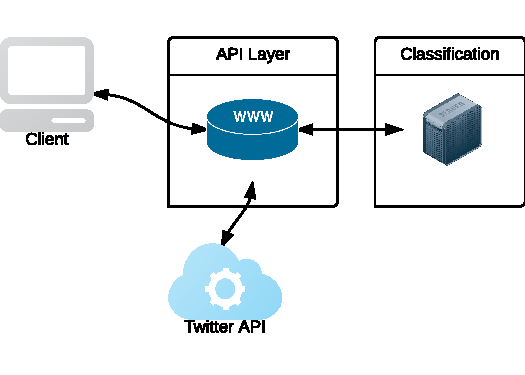
\includegraphics[width=0.8\textwidth]{../img/NetworkDiagram.pdf}
 \end{center}
 \caption[Architectural overview of the system.]{Architectural overview of the system. The client retrieves data from the Twitter API and uses the classification server for sentiment classification.}
 \label{fig:NetworkDiagram.pdf}
\end{figure}

A client makes a request to the API Layer, with the same interface as the Twitter API service. From there the API Layer will retrieve information from the Twitter API with HTTP requests, iterate over all tweets received, and send them in parallel to the classification server. When the classification server is done processing and classifying the tweet, it is sent back to the API Layer. When the API layer has received all the tweets, it responds to the client with the same JSON structure as the Twitter API sends out, only with an additional attribute noting the tweet's sentiment. This architecture and application flow can be seen in~\autoref{fig:NetworkDiagram.pdf}. 

\subsection{API Layer Extension}

To be able to have a scalable and responsive solution, the API Layer was written using the Node.js platform. Since Node.js uses JavaScript as programming language, the JSON data retrieved from the Twitter REST and Streaming API are easily manipulated and passed around. 

The API Layer works as a thin layer extending the Twitter API. This means that the interface used by Twitter, with all defined options and appropriate methods, is reflected through the API Layer. The main benefit is that all documentation for the Twitter API also documents most of this extended API Layer.

For authentication, an application is registered with a developer account at the Twitter Developer site. This creates OAuth credentials, which is used to identify the application, and to gain access to the Twitter data. For this implementation, the data is retrieved using the OAuth access for the application, not at user level. 

\subsubsection{Architectural Flow}


\begin{figure}[htb]
 \begin{center}
     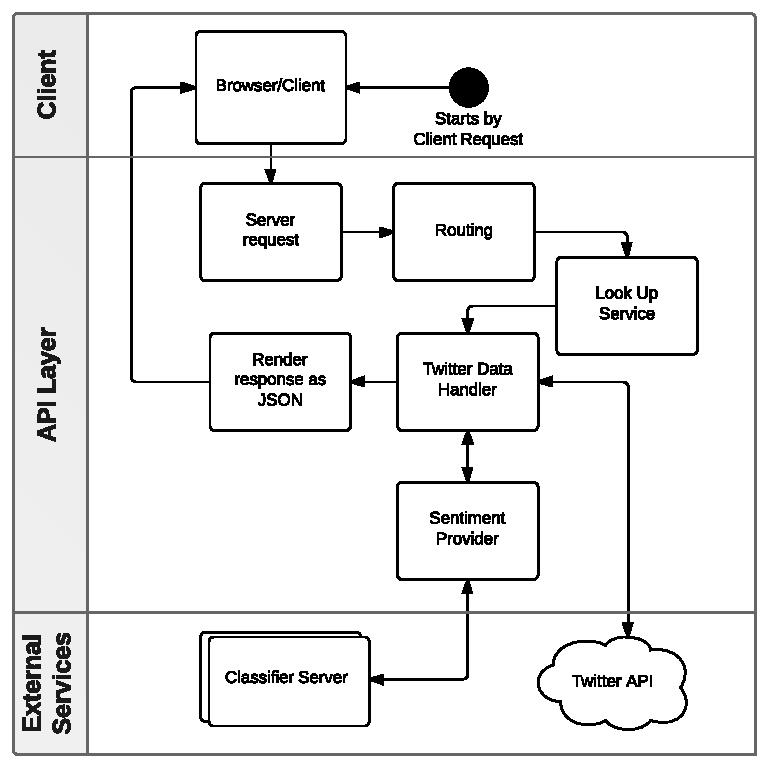
\includegraphics[width=0.8\textwidth]{../img/APILayerArcitechture.pdf}
 \end{center}
 \caption[Architectural overview of the API Layer.]{Architectural overview of the API Layer. A request is handled by the server, sending it to routing where it is processed and sent to service look-up. If a service is found, a request is sent to the Twitter API and the received data is extended by the Twitter Data Handler module to contain a sentiment. When all of the Twitter data are extended, the data is given as a response to the requesting client.}
 \label{fig:APILayerArcitechture.pdf}
\end{figure}

When a request from a client is made, the request gets processed by the server and the routing module determines what the client is looking for. When the proper service is found, the client-specified parameters are sent directly to the Twitter API, using the Twitter Data Handler module (TDH). The TDH module then iterates over all found tweets, and sends them in parallel to the classification server. When a tweet has been processed by the classification server the classified sentiment is sent back to the TBH module and the original tweet object is extended to contain a property with the sentiment. When all tweets are classified, the TBH module passes the extended twitter data to the render module. The render module renders the JSON data and sends it to the client with appropriate HTTP headers set. This application flow can be seen in~\autoref{fig:APILayerArcitechture.pdf}.

If there is an error during any part of the process, the error is caught by the routing module, and the error is rendered as a JSON object, in the same manner as it would be by the Twitter API. 

When using both the Twitter REST API and Streaming API, there is a high level of asynchronism. Especially when streaming, it is impossible to predict when the next tweet is received. Due to this the system designed needs to be able to handle this dynamic data flow. Node.js is an event-driven platform and has a natural support for asynchronous data. 

All internal and external message passing in the API Layer is asynchronous. When requesting Twitter for data, an event is triggered when that data is ready and all tweets are separately sent to the classifier. By sending all tweets separately in parallel, classification of the entire set of tweets does not take much longer than classifying only one tweet. 

When streaming, the TBH module opens a connection to the Twitter API, but never closes it. There is a continuously open connection to the Twitter server, which is feeding the TBH module with single tweets as they get stored in the Twitter system. From the first received tweet, a connection to the requesting client is opened by the render response module. This connection will also remain open. In this way there is an open connection between the client and the API Layer as well as between the API Layer and the Twitter API. The API Layer works as a middleman, taking in tweets, classifying them, and streaming them to the client. By running this entire process asynchronously, the system can process data independently of when it is published.


\subsection{Sentiment Analysis Classifier}
\label{sec:classifier_arch}

Python is computationally stronger than Node.js in many ways. Additionally, it is much more mature. There are a lot of well documented packages for handling various tasks. Scikit-learn (sklearn) is one of these packages. sklearn is package built on top of the Python packages numpy, scipy and matplotlib. sklearn integrates machine learning algorithms as SVM, NB, MaxEnt and more. sklearn implements solutions for doing feature extraction, grid searching, cross validation and a lot more for analysing text. Thus it is a good choice for the process of sentiment analysis. As a dynamic typed language, Python allows for rapid development and prototyping. These attributes are some of the reasons Python is a good fit for the present system. 

The Sentiment Analysis Classifier system runs as a server waiting for requests. The HTTP method POST is used for a client to send a \textit{stringified} tweet object to the server. Stringify is a JSON method for returning a serialized object represented by a string. The classification server converts this string to a Python dictionary. The response will be a string with the sentiment classification, that is, either \textit{positive}, \textit{neutral} or \textit{negative}. The classification scheme can be extended if necessary. 

The classifier server can be initialized with different settings for classification strategy, what port to run at, what training data to use, and whether or not to show debug data. This allows for multiple servers running at the same time, with different settings. Running multiple server instances makes it easier to compare different classification strategies. Two servers could run side by side, and a test framework could use the two servers to classify the same tweets for a comparison.

When the server is initiated, the selected model is trained by having and made availeble to be used by the classification server. 

The classification server uses a pool of child processes. For each receiving tweet, it spawns a new child from this pool and in this process the tweet is classified. This way the classification server can process several tweets in parallel, which helps the one-to-one relationship between a tweet on the classification server and the same tweet on the API Layer.

\subsubsection{Architectural Flow}

\begin{figure}[htb]
 \begin{center}
     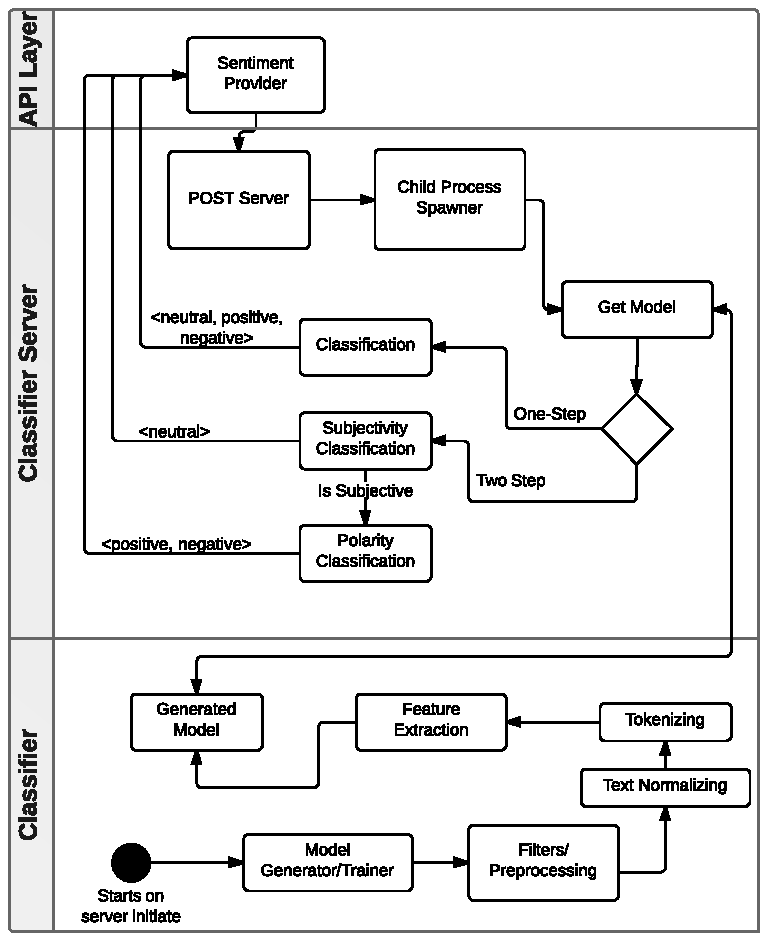
\includegraphics[width=0.8\textwidth]{../img/ClassifierArcitechture30.pdf}
 \end{center}
 \caption[Architectural overview of the classification server.]{Architectural overview of the classification server. On server start, a model for predicting seniment is generated. When a request from the API Layer is made to the POST Server, a child processes is spawned. The tweet text is extracted and sent into the model for classification. If the classification model is a one-step process, the classifier returns to the sentiment provider with either a neutral, positive or negative classification. If the generated model is two-stepped, the tweet is first classified as either neutral or subjective. If it is neutral, it is returned to the API Layer, if it is subjective, it is sent to the next step and the result from that step is returned to the sentiment provider.}
 \label{fig:ClassifierArcitechture}
\end{figure}

\begin{figure}[htb]
 \begin{center}
     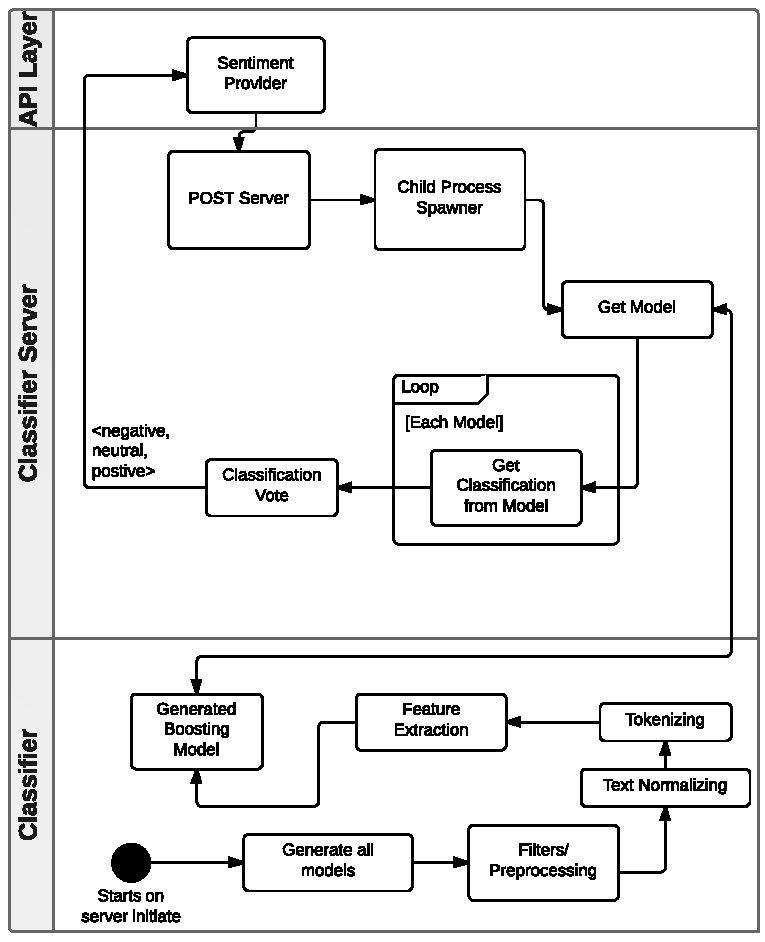
\includegraphics[width=0.8\textwidth]{../img/ClassifierArcitechture30Boosting.pdf}
 \end{center}
 \caption[Architectural overview of the classification server with Boosting.]{Architectural overview of the classification server with boosting. On server start, the Boosting model for predicting seniment is generated with a set of sub-models. When a request from the API Layer is made to the POST Server, a child processes is spawned. The tweet text is extracted and sent into the model for classification. All models predicts a sentiment and sends the sentiment to voting. For voting the Boosting model selects the sentiment with highest score and returns this to the API sentiment provider.}
 \label{fig:ClassifierArcitechtureBoosting}
\end{figure}

The Sentiment Provider module from the API Layer makes a request to the classifier's POST Server. The POST server translates the string to a Python dictionary and passes the information down to the Child Process Spawner. A new process is spawned and, using the module generated when initiating the server, the tweet is classified and returned to the API Layer.

When the classification model is trained on the server initialization, various text filters, normalizations and other pre-processing methods can be utilized, as seen in figure~\ref{fig:ClassifierArcitechture}. The model can be generated as either a one-step process, two-step process or a combination using Boosting. 

If a one-step model is used, one algorithm is used to classify the tweet as either negative, neutral or positive. If a two-step model is used, the tweet is first classified as either subjective or neutral in the subjectivity classification step. If it is neutral, the model returns with the classification. If the result is subjective, the tweet is sent to the polarity classification step, where the result can either be negative or positive. The end classification is returned to the API Layer.

When using the Boosting model, a set of sub-models is generated and all used in conjunction to predict a sentiment of a tweet. All sub-models predicts and sends the classification to a voting mechanism. The final classification is the result of the vote. This process is visualized in figure~\ref{fig:ClassifierArcitechtureBoosting}.

\subsubsection{Classification Model Structure}

The classification models are implemented by wrapping machine learning algorithms from sklearn in a inheritance based class structure. By having every model inherit from a base model, the interface is the same across every model, and the system can use the model without having knowledge what kind of algorithm it uses. An overview of this structure is presented in figure~\ref{fig:ModelsStructure}.

The base parent model implements methods for training the machine learning algorithm and for predicing either a set of documents or one document. For simple algorithms as NB, SVM and MaxEnt, these generic methods can be used, but the TwoStep and Boosting model have their own implementation. 
 
\begin{figure}[htb]
 \begin{center}
     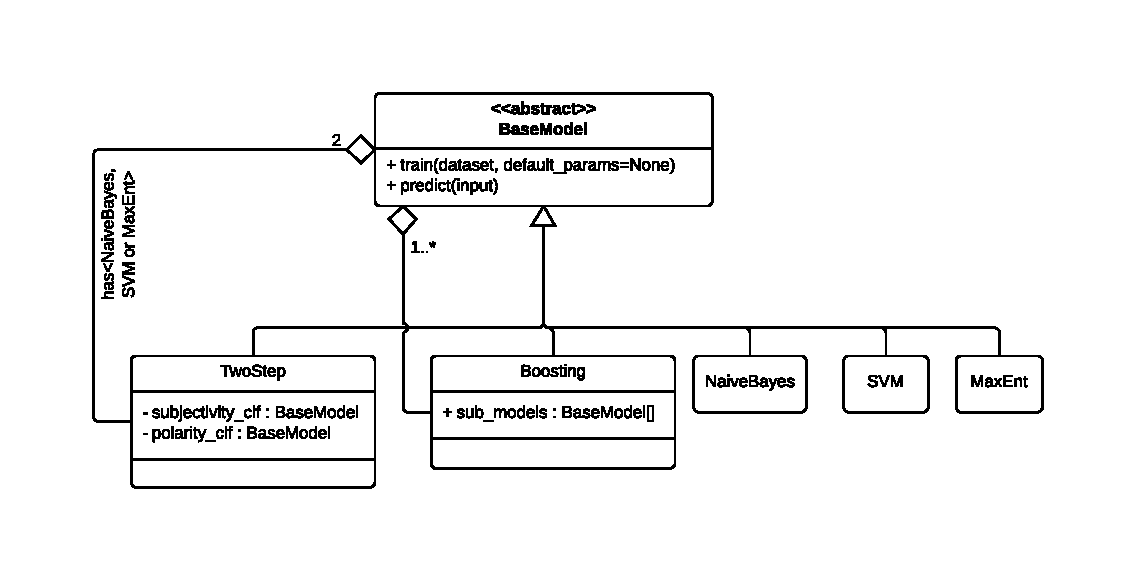
\includegraphics[width=0.8\textwidth]{../img/ModelsStructure.pdf}
 \end{center}
 \caption[Classification Model Structure Overview]{Overview of how the models are built and connected. There is a base model class implementing a method for predicing and training. All models extends from this base model. The models for NaiveBayes, SVM and MaxEnt uses the base model's implementation of train and predict, whilst the TwoStep and Boosting models implement their own. The interface for each model is the same.}
 \label{fig:ModelsStructure}
\end{figure}


\section{Visualization Applications}
\label{sec:visualization_applications}
To test and give example of how to use the generic system designed in~Section\ref{sec:tsaarchitecture}, different visualization applications were implemented. Each of these applications is described in their own sub section in this section. The sub sections are divided into describing how the applications are implemented and the finished product.

\subsection{SentiMap: Geo-location based streams}

\subsubsection{Implementation}

\subsubsection{Product}

\begin{figure}[htb]
\begin{center}
 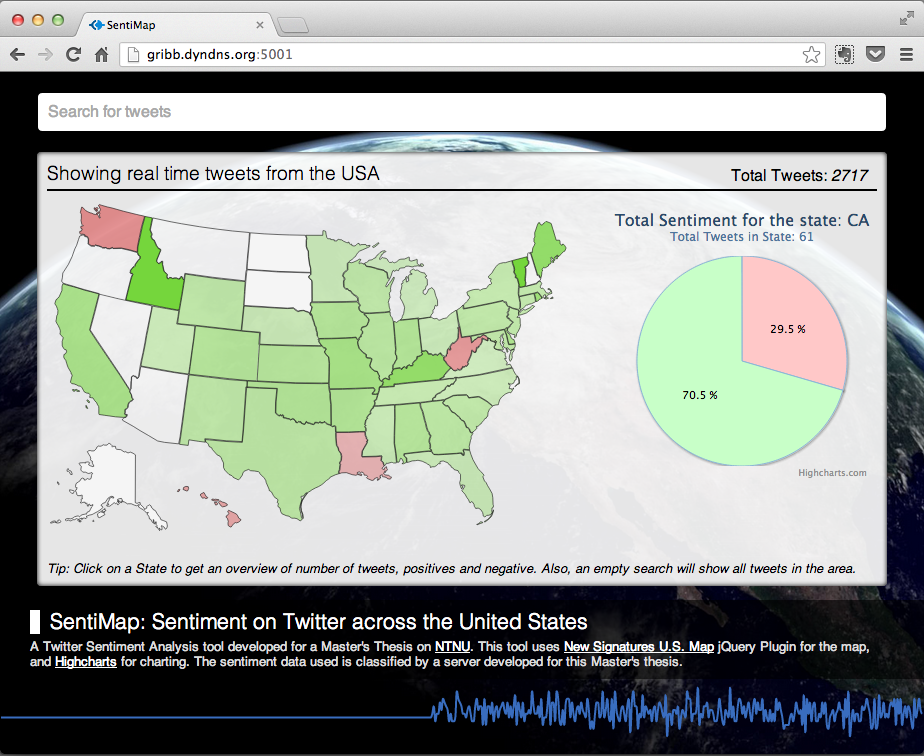
\includegraphics[width=0.8\textwidth]{../img/sentimap_screenshot.png}
 \caption{Screen shot of the SentiMap system running.}
 \label{fig:sentimap_screenshot}
\end{center}
\end{figure}

\begin{figure}[htb]
\begin{center}
 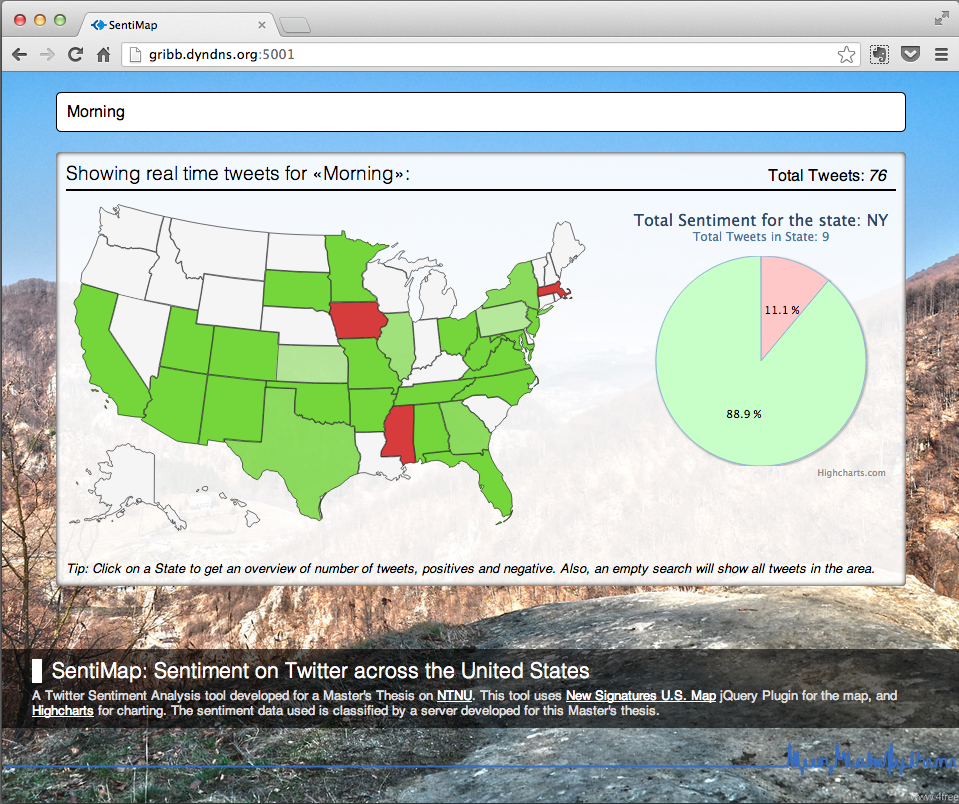
\includegraphics[width=0.8\textwidth]{../img/sentimap_screenshot_search.png}
 \caption{Screen shot of the SentiMap when searching for a query.}
 \label{fig:sentimap_screenshot_search}
\end{center}
\end{figure}

\begin{figure}[htb]
\begin{center}
 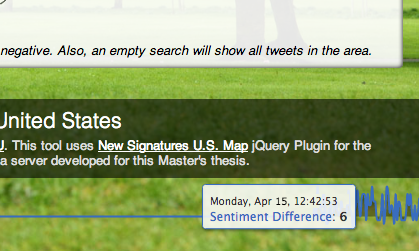
\includegraphics[width=0.6\textwidth]{../img/sentimap_screenshot_timeline.png}
 \caption[SentiMap timeline screen shot]{Showing the sentiment difference (positive minus negative sentiments) on that exact second from the streamed data.}
 \label{fig:sentimap_screenshot_timeline}
\end{center}
\end{figure}

\subsection{Tweet Searching}



\chapter{Experiments and Results}

This should most likely contain both the results from the classification task and the visualization task.

\textcolor{blue}{(8-10 pages) In this chapter you present your results from your work, coming from 
testing/validating/exploring the theory/research-questions by empirical studies. It can be structured by contributions, 
research questions, or studies done. Find what suits your thesis and results. Some also like to include the 
bibliography of the included papers with abstract and identified contributions towards the thesis. Do not use all of 
the headlines below, if it leads to the same point being said over and over. Find the approach that best makes your 
point.}

\section{Developer Tools}
\textcolor{blue}{Describe what system and tools we use for the experiments}


\section{Description of Experiment}
\textcolor{blue}{Describe how the experiment was conducted.}

To experiment with different solutions for sentiment analysis, a system testing platform and code base was developed. This testing system generates and trains different models based on input arguments as default values for algorithms and type of algorithm. The architecture and flow of this system is described as a part of section~\ref{sec:classifier_arch}.

The testing system can take in a set of parameters to use for an algorithm, like pre-processor methods, whether or not to use inverse document frequency (IDF) or stop words and so on, or a grid search flag can be set. If the grid search option is activated, a model is generated with the best possible parameters set for the given algorithm. The grid search is conducted using cross validation, and the set of parameters to search across. The parameter search space is reflected in table~\ref{tab:gridsearch_params}.


\subsection{Pre-processing and Feature Selection}

\begin{table}[htb]
	\centering
	\begin{tabular}{|r||c|c|c|c|c|c|c|c|}
		% P1  -> no\_usernames
		% P2 -> remove\_noise
		% P3 -> placeholders
		% P4 -> all
		% P5 -> remove\_all
		% P6 -> reduced\_attached
		% P7 -> no\_url\_usernames \_reduced \_attached

		\cline{2-9}
	 \multicolumn{1}{c| }{ } & \textbf{None} & \textbf{P1} & \textbf{P2} & \textbf{P3} & \textbf{P4} & \textbf{P5} & \textbf{P6} & \textbf{P7}  \\ \hline
		Remove Usernames                     & & x & x &   & x & x & & x \\ \hline
		$||U||$ instead of $@username$       & &   &   & x &   &   & & \\ \hline
		Remove URLs                          & &   & x &   & x & x & & x \\ \hline
		$||URL||$ instead of real URL        & &   &   & x &   &   & & \\ \hline
		Remove Hash-tags                     & &   &   &   & x & x & & \\ \hline
		Hash-tags as words                   & &   & x &   &   &   & & \\ \hline
		$||H||$ instead of hash-tag          & &   &   & x &   &   & & \\ \hline
		Remove $RT$-tag                      & &   & x &   & x & x & & \\ \hline
		Remove emoticons                     & &   &   &   & x & x & & \\ \hline
		Reduce letter duplicates             & &   & x &   & x &   & x & x \\ \hline
		Attach negation to surrounding words & &   &   &   & x &   & x & x \\ \hline
	\end{tabular}
	\caption[Description of used pre-processing methods]{Description of the pre-processing methods used for the experiments. Some functions remove entities, other replace them with a place holder text. The hash-tag as word transforms a hash-tag to a regular word and uses the hash-tag as a feature. "Reduce letter duplicates", reduces redundant letters to a maximum of three.}
	\label{tab:preproc_desc}
\end{table}

\subsubsection{Removing features}

\subsubsection{Replacing with place holders}

\subsubsection{Reducing letter duplication}

\subsubsection{Attaching negation}

\begin{table}[htb]
\centering
\begin{tabular}{|r||c|c|c|} 
\cline{2-4}

\multicolumn{1}{c|}{ } & \textbf{NB} & \textbf{SVM} & \textbf{MaxEnt} \\ \hline
alpha & <0.1, 0.3, 0.5, 0.7, 0.8, 1.0> & \multicolumn{2}{ c| }{-} \\ \hline
penalty  &  - &  - & L1 or L2 \\ \hline
C &  - & \multicolumn{2}{ c| }{<0.1, 0.3, 0.5, 0.7, 0.8, 1.0>} \\ \hline
ngram &  \multicolumn{3}{ c| }{ Unigram, Bigram or Trigram } \\ \hline
Use IDF &  \multicolumn{3}{ c| }{ Yes or No } \\ \hline
Use Smooth IDF &  \multicolumn{3}{ c| }{ Yes or No } \\ \hline
Use Sublinear IDF &  \multicolumn{3}{ c| }{ Yes or No } \\ \hline

\end{tabular}
\caption{Overview of parameter search space for the grid searches conducted in the experiments.}
\label{tab:gridsearch_params}
\end{table}

\begin{figure}[htb]
	\centering
	\begin{tikzpicture}
	  \begin{axis}[
	    ybar,
	    enlargelimits=0.15,
	    legend style={at={(0.5,-0.2)},
	      anchor=north,legend columns=-1},
	    ylabel={\# times used},
	    symbolic x coords={P2,P7,P6, P1,P3},
	    xtick=data,
	    nodes near coords, 
		nodes near coords align={vertical},
	    x tick label style={rotate=45,anchor=east},
	    ]
	    \addplot coordinates {(P2,10) (P7,4) 
			(P6,3) (P1,3) (P3,1)};
	  \end{axis}
	\end{tikzpicture}
	\label{fig:preprocess_usage}
	\caption[Statistics of pre-processing usage.]{Statistics of pre-processing usage. Removing all usernames, urls hash-tag character, RT-tag and excessive letters as features seem to perform the best.}
\end{figure}

\section{Experiment Results}
\textcolor{blue}{Show plots, significant features and so on and describe the results from the experiment}

\subsection{Grid Search}
As described above, an extensive grid search was conducted. This search cycled through different algorithms, parameters and preprocessing techniques. Figure~\ref{fig:results_full} displays the precision, recall, F-measure and accuracy for each of the classifiers with test set 1 as evaluation data. We notice that most of the classifiers that includes the NB algorithm has a bad performance, both for accuracy and F-measure. This was observed for other test sets as well. Further, we can see that the MaxEnt classifier has the best accuracy, while SVM has a slightly better F-measure.

We can also see that all the classifiers with SVM tends to give a better cofusion matrix than the others. This is showed in Figures (firstconf - lastconf).

\subsubsection{Parameters and options}
As a part of the grid search, the system tried to apply all the different preprocessing methods for each classifier. Figure~\ref{fig:preprocess_usage} clearly shows that P2 (removing user names, URLs, hash-tag prefixes, RT-tokens and redundant letters) is the preprocessing method that was used most often, i.e., it gave the best accuracy. Figure~\ref{fig:preprocess_usage} also indicates that URLs are noisy, and does not contain any sentiment, and that hash-tags and emoticons are valuable features.


Notes:
\begin{enumerate}
\item Grid search across params result in MaxEnt being the best. With following params:
	\begin{itemize}
		\item 'ngram\_range': (1,1),
		\item  'sublinear\_tf': True,
		\item  'preprocessor': P3,
		\item  'use\_idf': True,
		\item  'smooth\_idf': True,
		\item  'max\_df': 0.5,
		\item  'stop\_words': None
	\end{itemize}
	\begin{itemize}
		\item 'C': 1.0,
		\item 'penalty': 'l1'
	\end{itemize}
	
\item Best impl has a accuracy of 0.645, but a bad confusion matrix.

\item SVM also performs well (probably better). Best params:
	\begin{itemize}
		\item 'ngram\_range': (1,1),
		\item  'sublinear\_tf': True,
		\item  'preprocessor': P2,
		\item  'use\_idf': True,
		\item  'smooth\_idf': True,
		\item  'max\_df': 0.5,
		\item  'stop\_words': None
	\end{itemize}
	\begin{itemize}
		\item 'C': 0.3
	\end{itemize}

\item Best impl of SVM has a accuracy of 0.638, better confusion matrix than MaxEnt

\item Overall stats for feature filters:
	\begin{description}
		\item[remove\_noise] 10
		\item[no\_url\_usernames\_reduced\_attached] 4
		\item[placeholders] 1
		\item[reduced\_attached] 3
		\item[no\_usernames] 3
	\end{description}

\item SVM uses remove\_noise (P2) and MaxEnt is the only one using placeholders (P3). 
 
\item Can see that even though maxent scored better, it has a worse confusion matrix, than SVM. Not much difference in accuracy really. 

\item SVM and MaxEnt is performs much better than the rest. 
\end{enumerate}

Some other text... 

\begin{sidewaysfigure}[htb]
 \begin{center}
     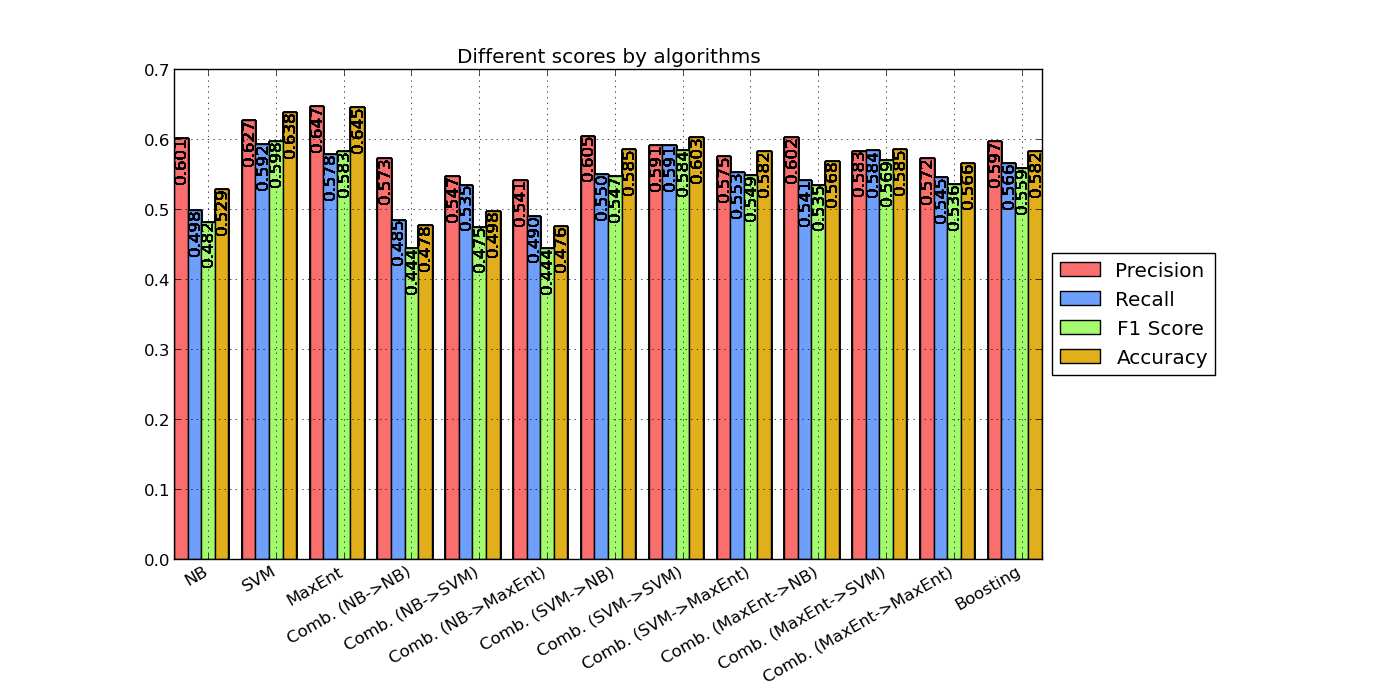
\includegraphics[width=\linewidth]{../img/plots/grid/full.png}
 \end{center}
 \caption[Results overview across models]{Caption description over here.}
 \label{fig:results_full}
\end{sidewaysfigure}



\begin{minipage}[s]{\linewidth}
     \centering
     \begin{minipage}{0.45\linewidth}
          \begin{figure}[H]
               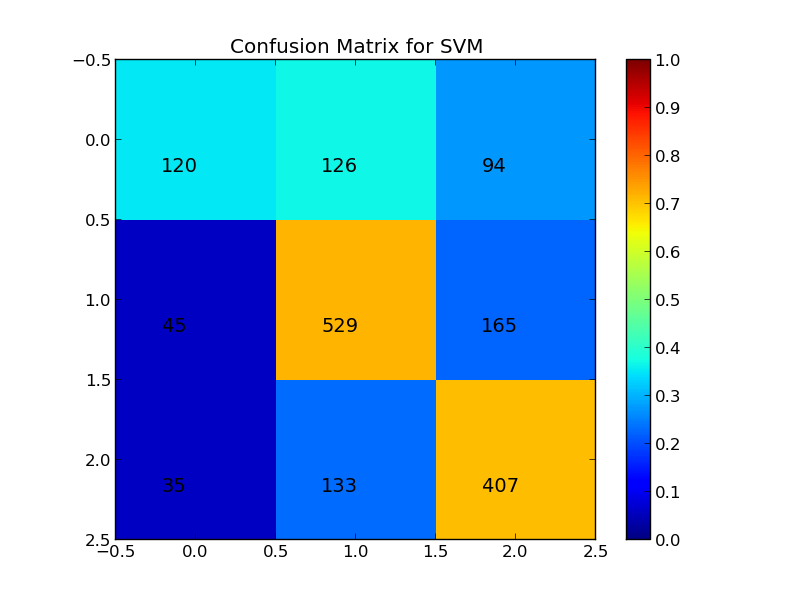
\includegraphics[width=\linewidth]{../img/plots/grid/confusion_matrix_SVM.png}
           \caption[Results overview across models]{Caption description over here.}
           \label{fig:confmat_svm}
          \end{figure}
     \end{minipage}
     \hspace{0.05\linewidth}
     \begin{minipage}{0.45\linewidth}
          \begin{figure}[H]
               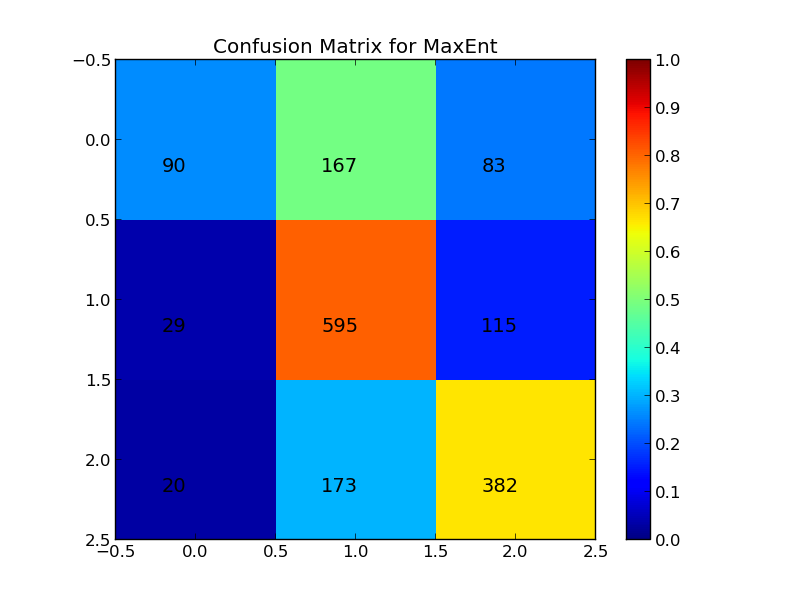
\includegraphics[width=\linewidth]{../img/plots/grid/confusion_matrix_MaxEnt.png}
           \caption[Results overview across models]{Caption description over here.}
           \label{fig:confmat_maxent}
          \end{figure}
     \end{minipage} \\
 
     \begin{minipage}{0.45\linewidth}
          \begin{figure}[H]
               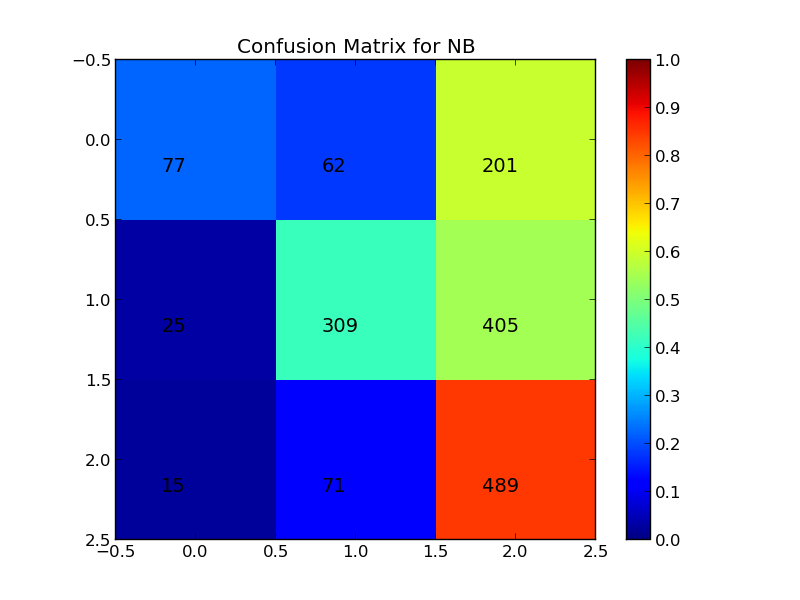
\includegraphics[width=\linewidth]{../img/plots/grid/confusion_matrix_NB.png}
           \caption[Results overview across models]{Caption description over here.}
           \label{fig:confmat_nb}
          \end{figure}
     \end{minipage}
     \hspace{0.05\linewidth}
     \begin{minipage}{0.45\linewidth}
          \begin{figure}[H]
               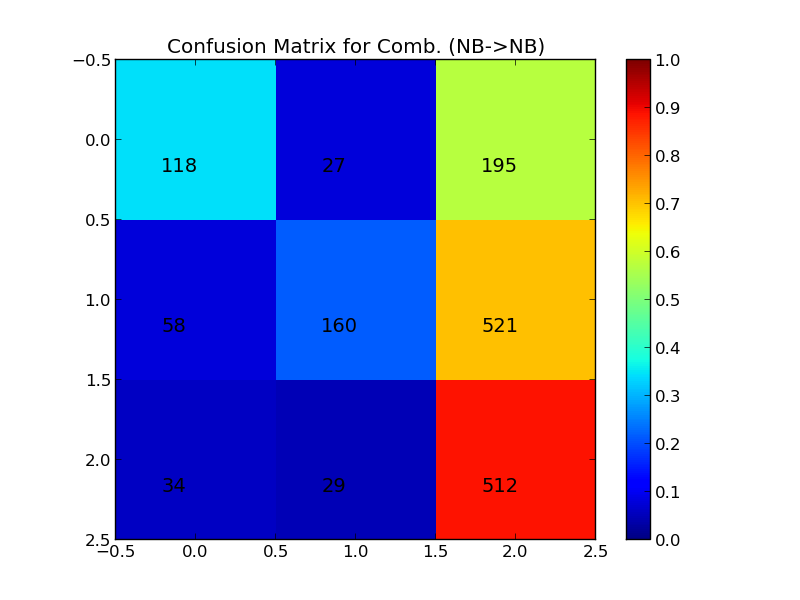
\includegraphics[width=\linewidth]{../img/plots/grid/confusion_matrix_Comb-NB-NB.png}
           \caption[Results overview across models]{Caption description over here.}
           \label{fig:confmat_nb_nb}
          \end{figure}
     \end{minipage}   \\
         

     \begin{minipage}{0.45\linewidth}
          \begin{figure}[H]
               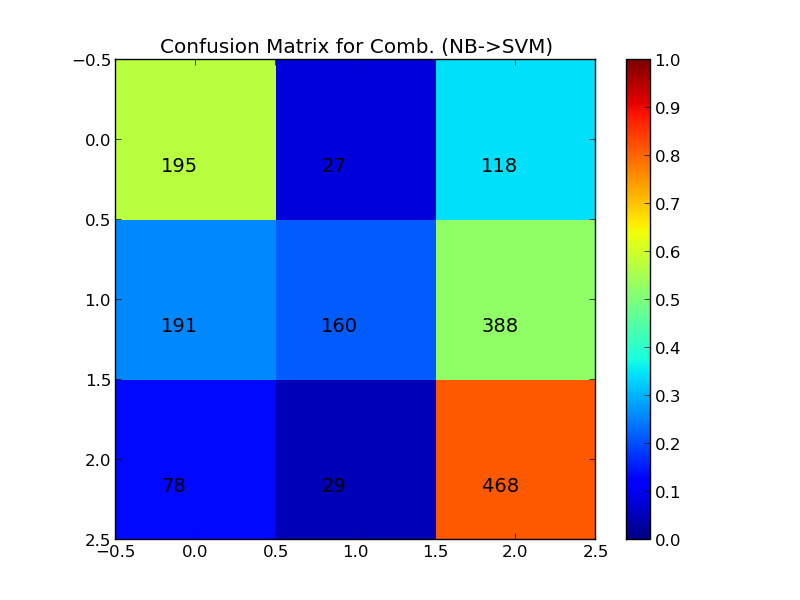
\includegraphics[width=\linewidth]{../img/plots/grid/confusion_matrix_Comb-NB-SVM.png}
           \caption[Results overview across models]{Caption description over here.}
           \label{fig:confmat_nb_svm}
          \end{figure}
     \end{minipage}
     \hspace{0.05\linewidth}
     \begin{minipage}{0.45\linewidth}
          \begin{figure}[H]
               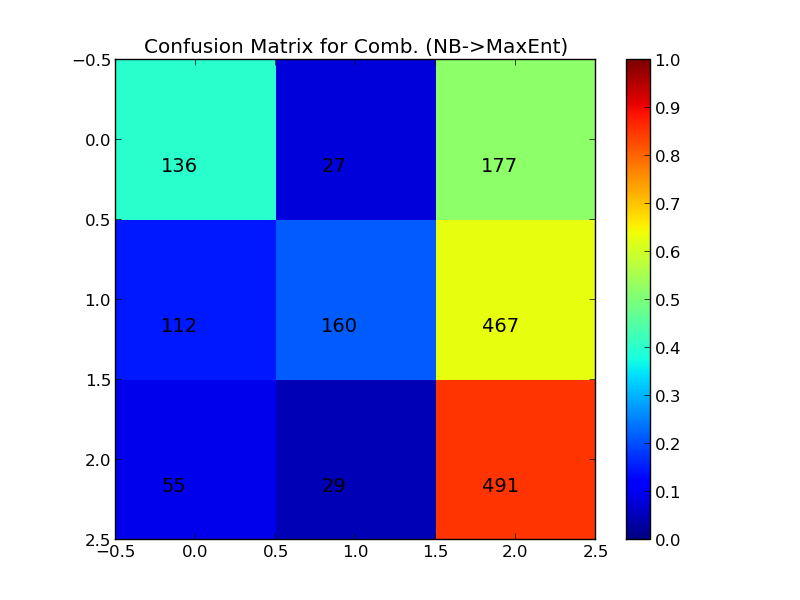
\includegraphics[width=\linewidth]{../img/plots/grid/confusion_matrix_Comb-NB-MaxEnt.png}
           \caption[Results overview across models]{Caption description over here.}
           \label{fig:confmat_nb_maxent}
          \end{figure}
     \end{minipage}
\end{minipage}


\begin{minipage}[s]{\linewidth}
     \centering
     \begin{minipage}{0.45\linewidth}
          \begin{figure}[H]
               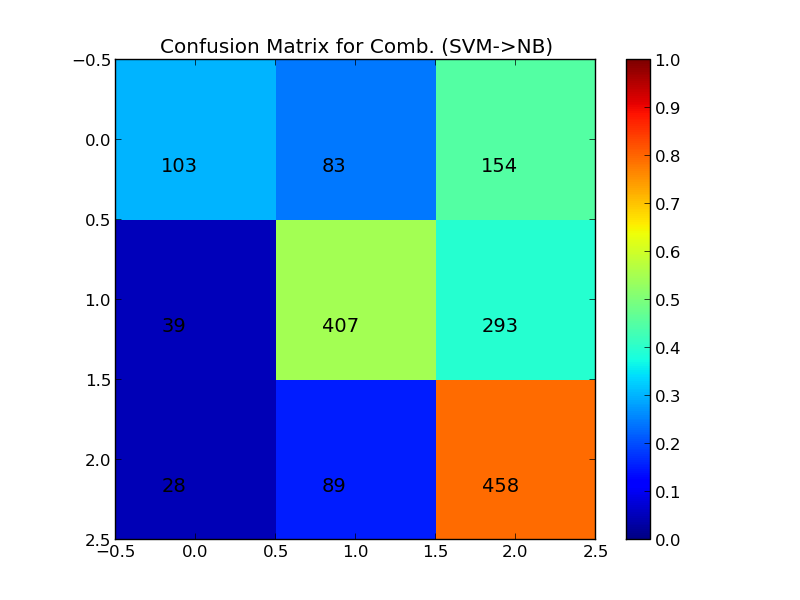
\includegraphics[width=\linewidth]{../img/plots/grid/confusion_matrix_Comb-SVM-NB.png}
           \caption[Results overview across models]{Caption description over here.}
           \label{fig:confmat_svm_nb}
          \end{figure}
     \end{minipage}
     \hspace{0.05\linewidth}
     \begin{minipage}{0.45\linewidth}
          \begin{figure}[H]
               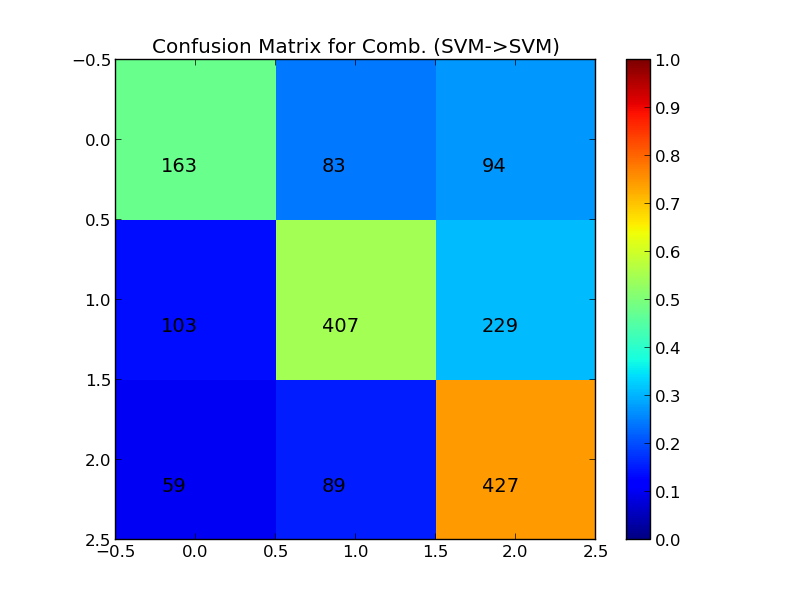
\includegraphics[width=\linewidth]{../img/plots/grid/confusion_matrix_Comb-SVM-SVM.png}
           \caption[Results overview across models]{Caption description over here.}
           \label{fig:confmat_svm_svm}
          \end{figure}
     \end{minipage} \\
 
     \begin{minipage}{0.45\linewidth}
          \begin{figure}[H]
               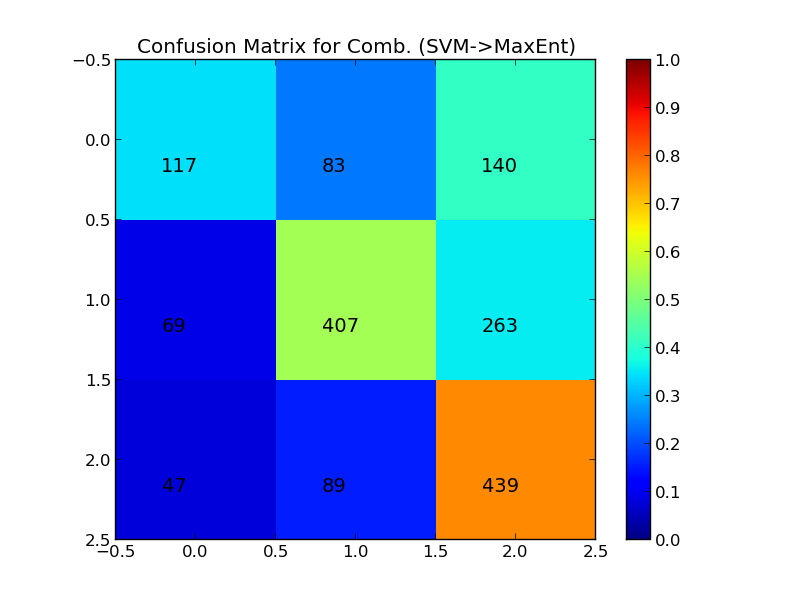
\includegraphics[width=\linewidth]{../img/plots/grid/confusion_matrix_Comb-SVM-MaxEnt.png}
           \caption[Results overview across models]{Caption description over here.}
           \label{fig:confmat_svm_maxent}
          \end{figure}
     \end{minipage}
     \hspace{0.05\linewidth}
     \begin{minipage}{0.45\linewidth}
          \begin{figure}[H]
               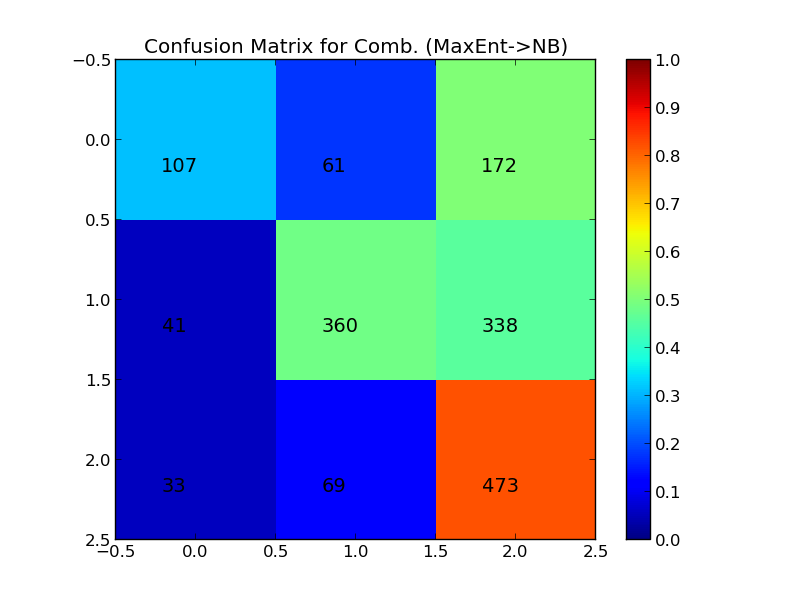
\includegraphics[width=\linewidth]{../img/plots/grid/confusion_matrix_Comb-MaxEnt-NB.png}
           \caption[Results overview across models]{Caption description over here.}
           \label{fig:confmat_maxent_nb}
          \end{figure}
     \end{minipage}   \\
         

     \begin{minipage}{0.45\linewidth}
          \begin{figure}[H]
               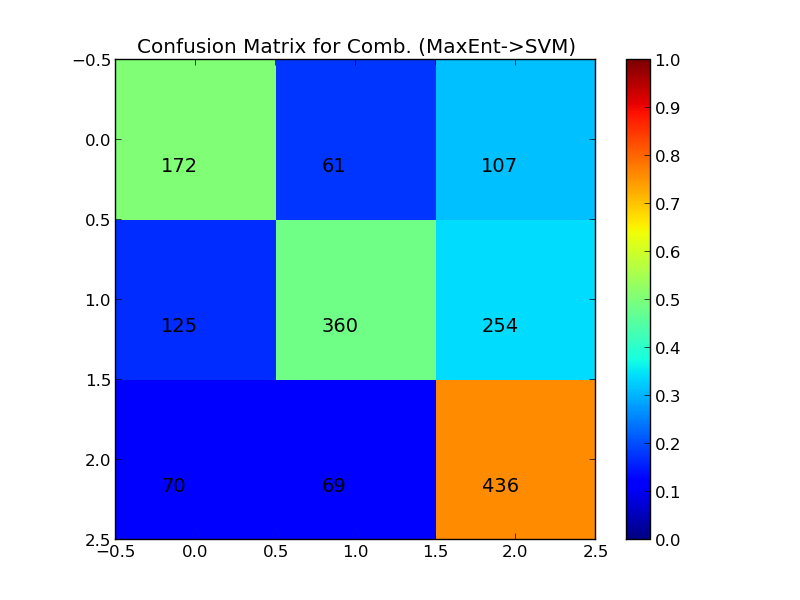
\includegraphics[width=\linewidth]{../img/plots/grid/confusion_matrix_Comb-MaxEnt-SVM.png}
           \caption[Results overview across models]{Caption description over here.}
           \label{fig:confmat_maxent_svm}
          \end{figure}
     \end{minipage}
     \hspace{0.05\linewidth}
     \begin{minipage}{0.45\linewidth}
          \begin{figure}[H]
               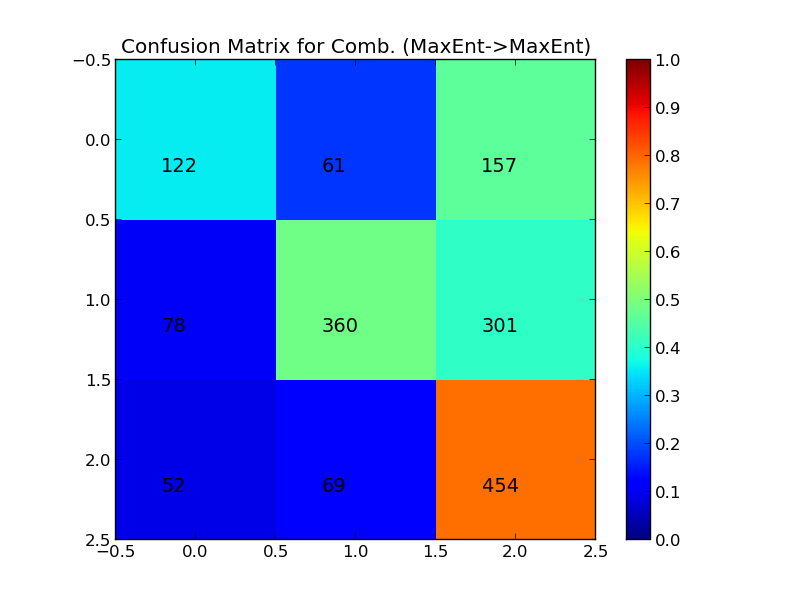
\includegraphics[width=\linewidth]{../img/plots/grid/confusion_matrix_Comb-MaxEnt-MaxEnt.png}
           \caption[Results overview across models]{Caption description over here.}
           \label{fig:confmat_maxent_maxent}
          \end{figure}
     \end{minipage}
\end{minipage}

\begin{figure}[H]
 \begin{center}
     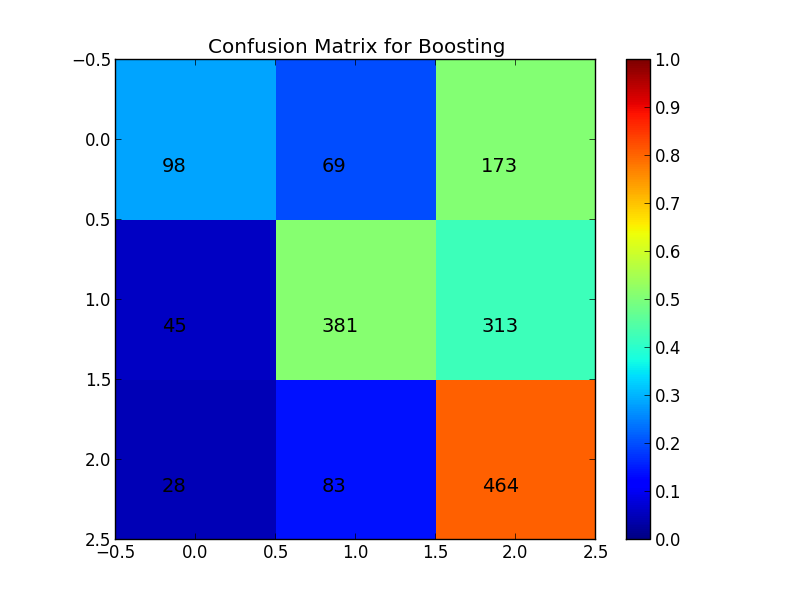
\includegraphics[width=0.7\linewidth]{../img/plots/grid/confusion_matrix_Boosting.png}
 \end{center}
 \caption[Results overview across models]{Caption description over here.}
 \label{fig:confmat_boosting}
\end{figure}


\begin{table}[htb]
\centering
\begin{tabular}{|r||c|c|c|} 
\cline{2-3}
\multicolumn{1}{c|}{ } & \textbf{SVM} & \textbf{MaxEnt} \\ \hline
ngram\_range & 1,1 & 1,1 \\ \hline
sunlinear\_tf  & True & True \\ \hline
preprocessor & P2 & P3 \\ \hline
use\_idf & True & True \\ \hline
smooth\_idf & True & True \\ \hline
max\_df & 0.5 & 0.5 \\ \hline
stop\_words & None & None \\ \hline
C & 1.0 & 0.3 \\ \hline
penalty & l1 & \\ \hline

\end{tabular}
\caption{Best parameters for SVM and MaxEnt.}
\label{tab:svm_maxent_best_params}
\end{table}



\begin{table}[!htb]
	
	\begin{minipage}{.45\linewidth}
		\begin{tabular}{|c|c|c|}
		
		\multicolumn{3}{c}{SVM} \\ \hline
		
		Negative & Neutral & Positive \\ \hline\hline
		
		no  		& wear & wait \\ \hline
		didn't  	& tallahassee & nice \\ \hline
		cancelled  	& 15th & interesting \\ \hline
		don't  		& 26 & awesome \\ \hline
		worse  		& at & cool \\ \hline
		why  		& trip & amazing \\ \hline
		bad  		& joe & fun \\ \hline
		worst  		& theres & ! \\ \hline
		hate  		& arrows & :) \\ \hline
		shit  		& murphy, & excited \\ \hline
		sad  		& question & happy \\ \hline
		sorry  		& plan & love \\ \hline
		not  		& set & best \\ \hline
		fuck  		& 8th & great \\ \hline
		:(  		& paterno & good \\ \hline
		\end{tabular}
	\end{minipage}
	\hspace{0.05\linewidth}
	\begin{minipage}{.45\linewidth}
		\begin{tabular}{|c|c|c|}

		
		\multicolumn{3}{c}{MaxEnt} \\ \hline
		
		Negative & Neutral & Positive \\ \hline\hline
		
		no 	& center & glad \\ \hline
		don't 	& royal & nice \\ \hline
		why 	& plan & thanks \\ \hline
		bad 	& joe & cool \\ \hline
		shit 	& nov & awesome \\ \hline
		injury 	& george & interesting \\ \hline
		cancelled 	& theres & amazing \\ \hline
		hate 	& arrows & :) \\ \hline
		worst 	& trip & fun \\ \hline
		worse 	& set & best \\ \hline
		fuck 	& question & excited \\ \hline
		sorry 	& at & love \\ \hline
		not 	& url & happy \\ \hline
		sad 	& 8th & good \\ \hline
		:( 	& paterno & great \\ \hline
		\end{tabular}
	\end{minipage}
	\caption[Most informative features]{Top 15 of the most informative features for SVM and MaxEnt}
	\label{tab:informative_features}
\end{table}



\section{NOTE: Analysis part: SVM vs MaxEnt}

\begin{figure}[htb]
	\centering
	\begin{minipage}{.45\linewidth}
		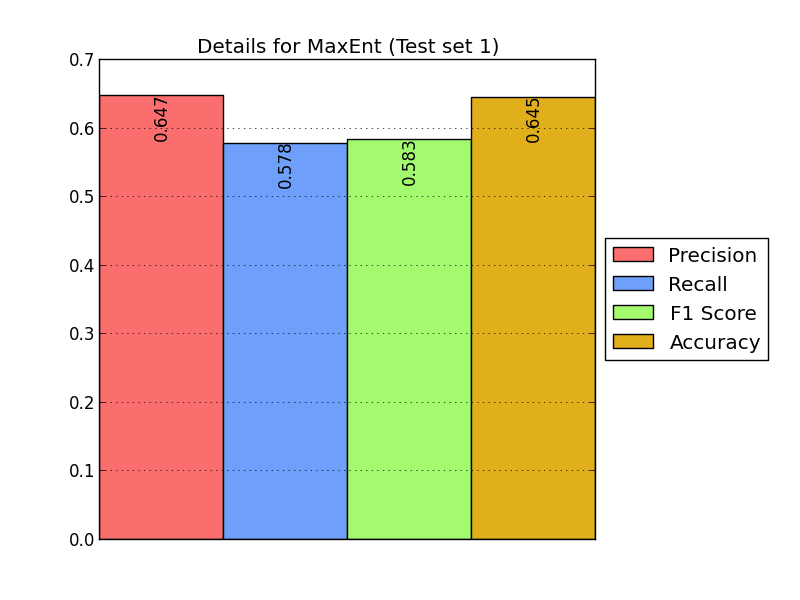
\includegraphics[width=\linewidth]{../img/plots/analysis/maxent_stats_best.png}
	\end{minipage}
	\hspace{0.05\linewidth}
	\begin{minipage}{.45\linewidth}
		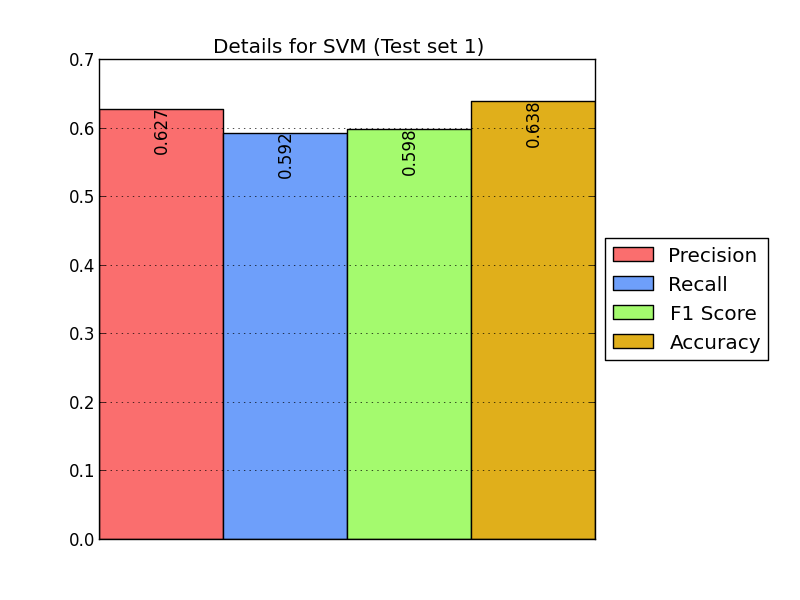
\includegraphics[width=\linewidth]{../img/plots/analysis/svm_stats_best.png}
	\end{minipage}
	\caption[Best performance plots for SVM and MaxEnt]{Best performance plots for SVM and MaxEnt}
	\label{fig:best_result}
\end{figure}

\begin{figure}[htb]
	\centering
	\begin{minipage}{.45\linewidth}
		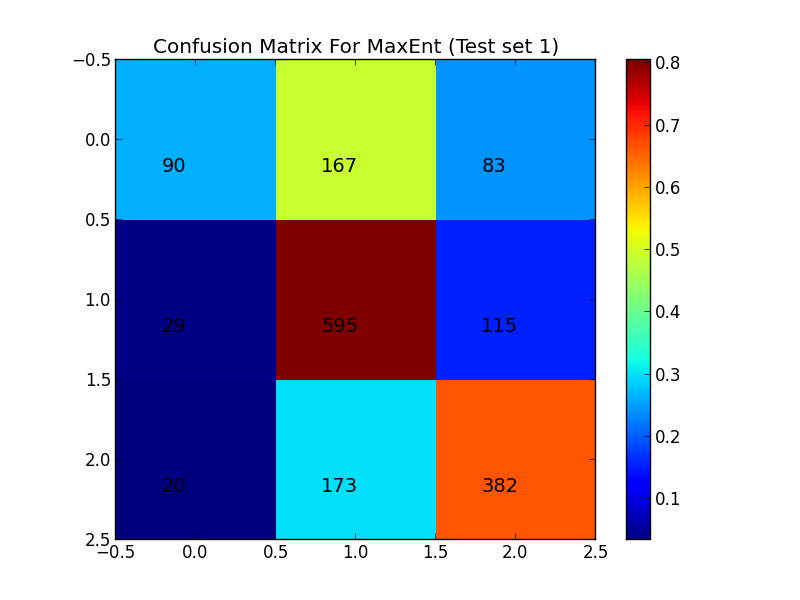
\includegraphics[width=\linewidth]{../img/plots/analysis/maxent_confusion_matrix_best.png}
	\end{minipage}
	\hspace{0.05\linewidth}
	\begin{minipage}{.45\linewidth}
		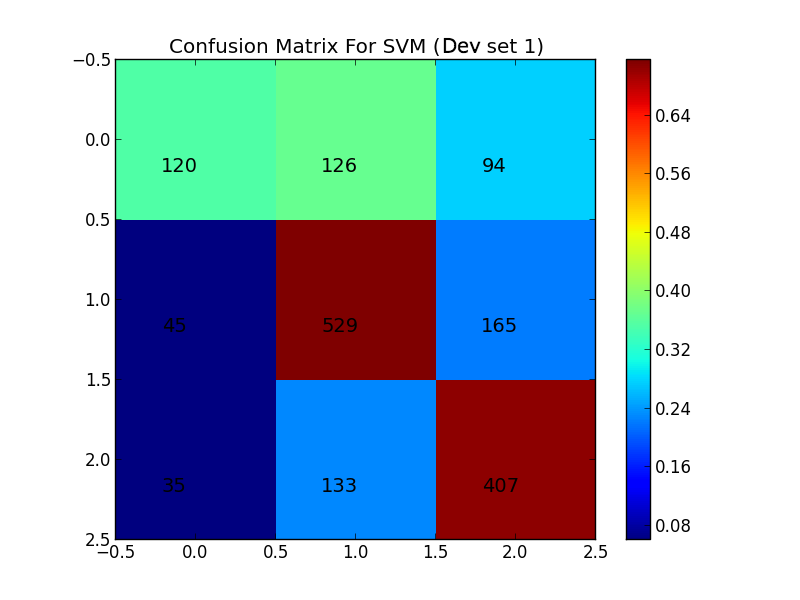
\includegraphics[width=\linewidth]{../img/plots/analysis/svm_confusion_matrix_best.png}
	\end{minipage}
	\label{fig:best_result_confusion}
	\caption[Confusion Matrix for SVM and MaxEnt]{Confusion Matrix for SVM and MaxEnt]}
\end{figure}





\begin{figure}[htb]
	\centering
	\begin{minipage}{.45\linewidth}
		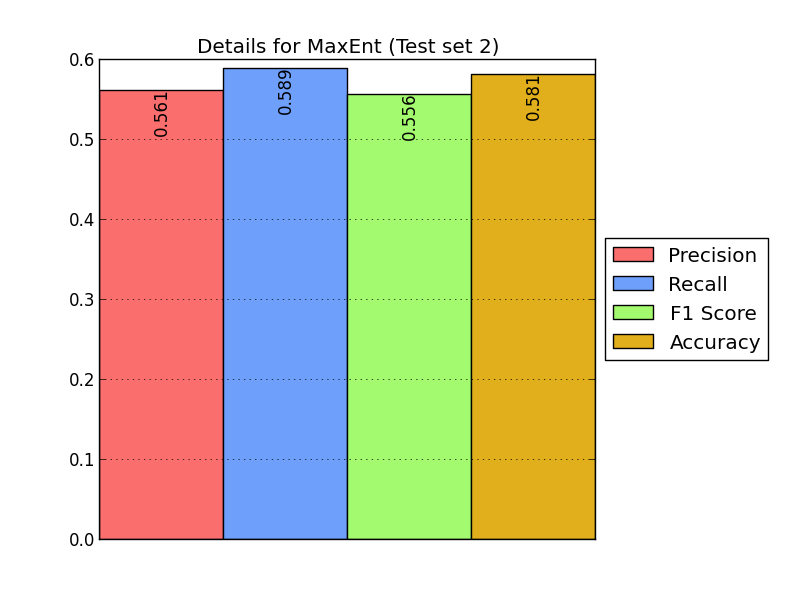
\includegraphics[width=\linewidth]{../img/plots/analysis/maxent_stats_best_diff_test.png}
	\end{minipage}
	\hspace{0.05\linewidth}
	\begin{minipage}{.45\linewidth}
		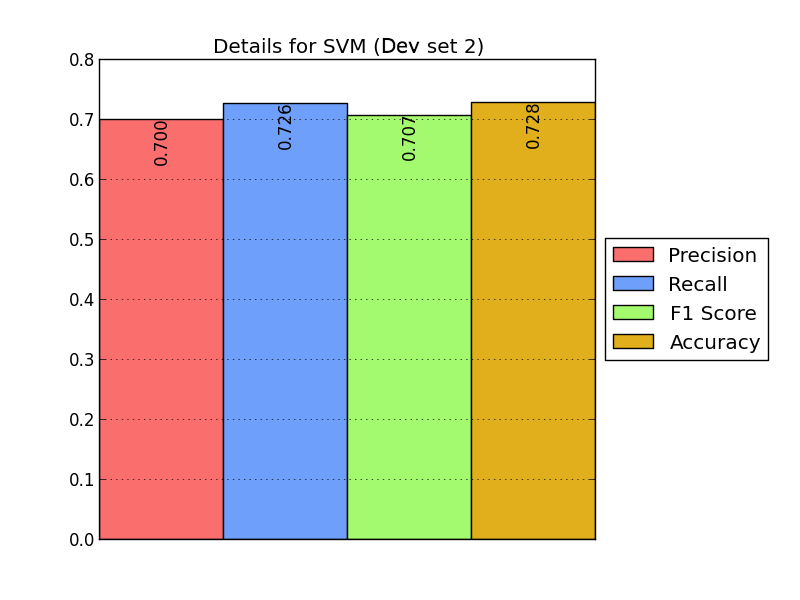
\includegraphics[width=\linewidth]{../img/plots/analysis/svm_stats_best_diff_test.png}
	\end{minipage}
	\label{fig:best_result_testset2}
	\caption[Best performance plots for SVM and MaxEnt for test set 2]{Best performance plots for SVM and MaxEnt using test set 2}
\end{figure}

\begin{figure}[htb]
	\centering
	\begin{minipage}{.45\linewidth}
		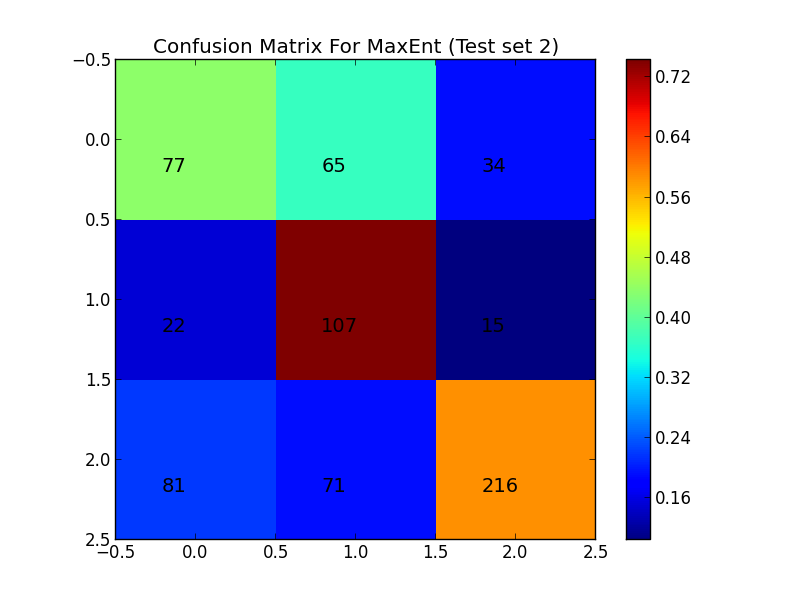
\includegraphics[width=\linewidth]{../img/plots/analysis/maxent_confusion_matrix_best_diff_test.png}
	\end{minipage}
	\hspace{0.05\linewidth}
	\begin{minipage}{.45\linewidth}
		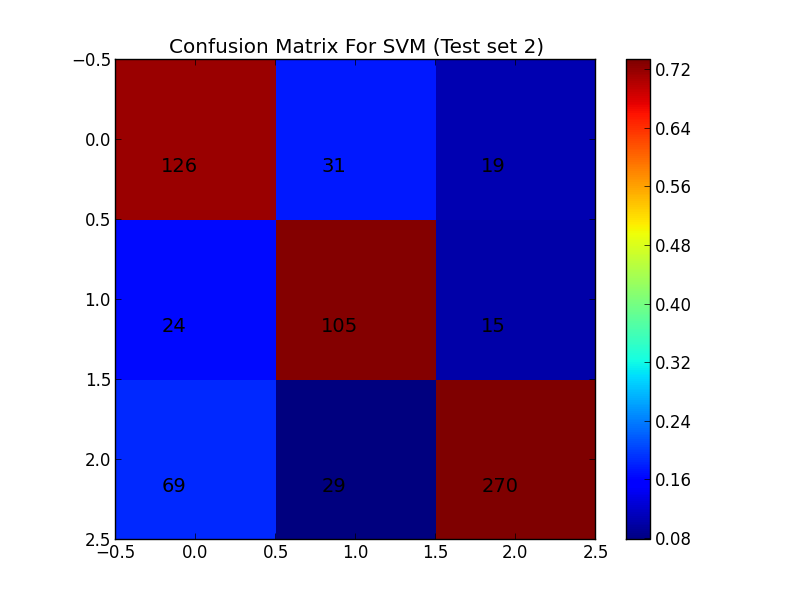
\includegraphics[width=\linewidth]{../img/plots/analysis/svm_confusion_matrix_best_diff_test.png}
	\end{minipage}
	\label{fig:best_result_confusion_testset2}
	\caption[Confusion Matrix for SVM and MaxEnt using test set 2]{Confusion Matrix for SVM and MaxEnt using test set 2}
\end{figure}



\begin{figure}[htb]
	\centering
	\begin{minipage}{.45\linewidth}
		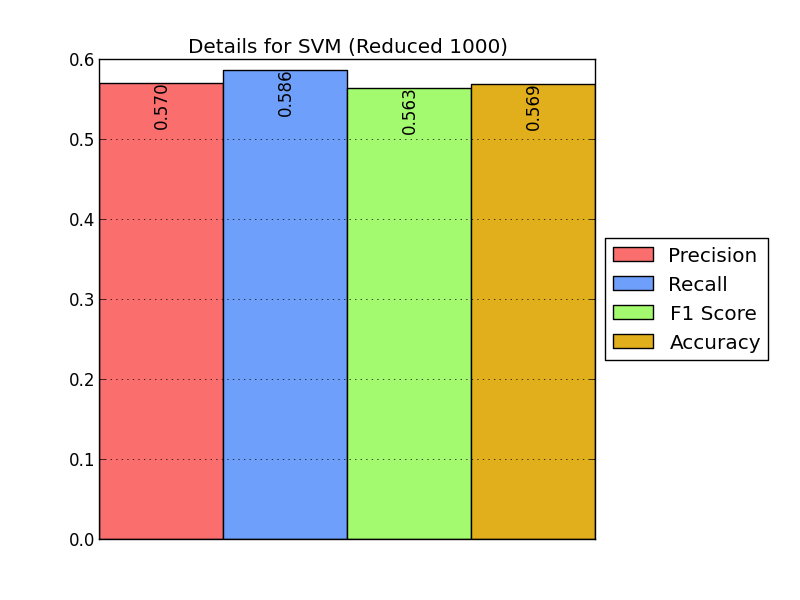
\includegraphics[width=\linewidth]{../img/plots/analysis/svm_stats_best_reduced_1000.png}
	\end{minipage}
	\hspace{0.05\linewidth}
	\begin{minipage}{.45\linewidth}
		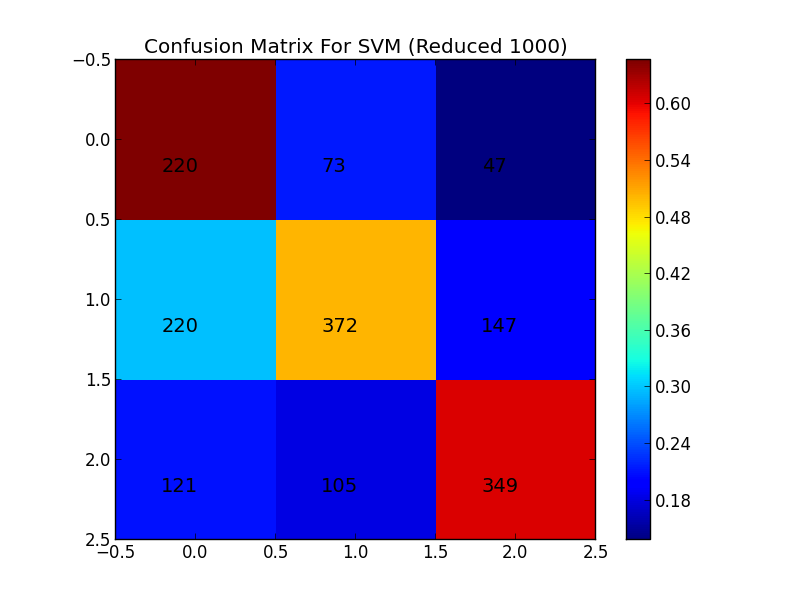
\includegraphics[width=\linewidth]{../img/plots/analysis/svm_confusion_matrix_best_reduced_1000.png}
	\end{minipage}
	\label{fig:svm_reduced_1000}
	\caption[Performance of SVM when reduced dataset to max 1000 per class]{Performance of SVM when reduced dataset to max 1000 per class}
\end{figure}

\begin{figure}[htb]
	\centering
	\begin{minipage}{.45\linewidth}
		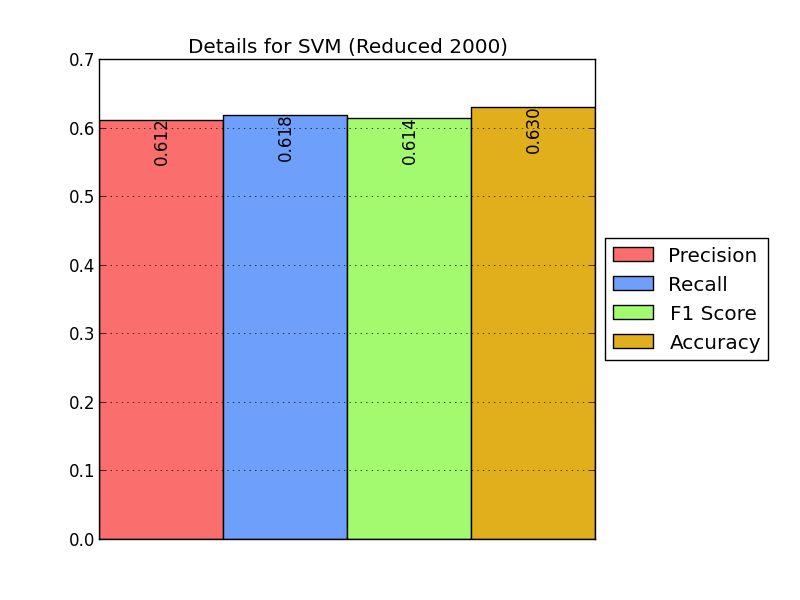
\includegraphics[width=\linewidth]{../img/plots/analysis/svm_stats_best_reduced_2000.png}
	\end{minipage}
	\hspace{0.05\linewidth}
	\begin{minipage}{.45\linewidth}
		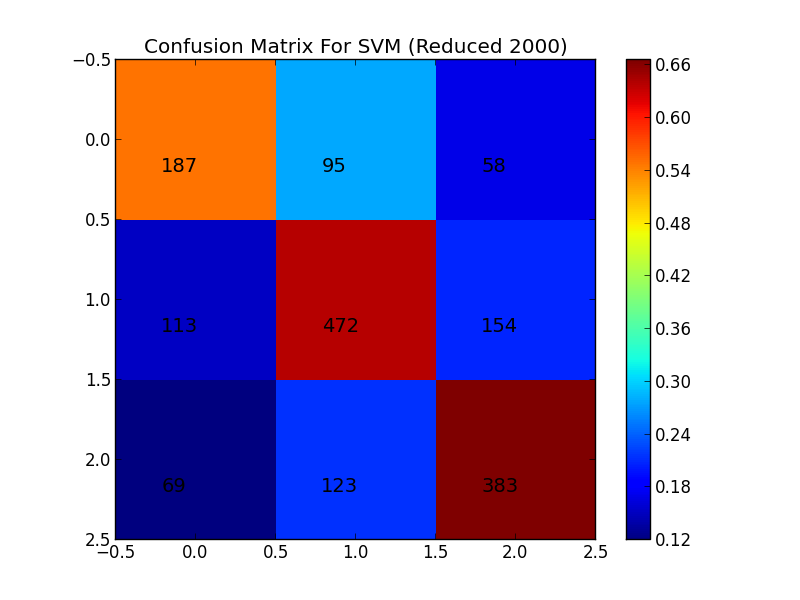
\includegraphics[width=\linewidth]{../img/plots/analysis/svm_confusion_matrix_best_reduced_2000.png}
	\end{minipage}
	\label{fig:svm_reduced_2000}
	\caption[Performance of SVM when reduced dataset to max 2000 per class]{Performance of SVM when reduced dataset to max 1000 per class}
\end{figure}

\chapter{Discussion}

In the introduction two main goals were introduced for this Master's Thesis:

\begin{description}

\item[G1] \textbf{Experiment with different models for doing sentiment analysis}
	
\item[G2] \textbf{Develop tools for visualising sentiment classified tweets}

\end{description}

This chapter will discuss whether or not we succeeded in reaching these goals, and discuss the solutions in general. The first section handles G1 and the second section discusses G2. The generic system architecture is an important part of achieving making the visualisation applications, and thus it is included in the latter section.

\section{G1: Experiment with different models for doing sentiment analysis}

In this section we will discuss whether we succeeded with our first goal or not, and how it was conducted. The first goal stated that we should try different models for classifying sentiment on short messages, such as tweets. 

The experiment description from~section~\ref{sec:experiment} show that we used grid searching on different machine learning algorithms and combination of algorithms to classify sentiment. A total set of 13 different models were thoroughly tested with a large training set. Our system generated graphs and plots comparing the different models, both on accuracy, F1-score, recall, precision and their confusion matrices. This comparative view allowed us to find what model performed best.

In our experiments we found that MaxEnt and SVM perform best in regards to accuracy. By conducting the experiments as stated, and finding the models with the highest accuracy, we succeed with the first goal.

The data that was used to train and evaluate the different models was given by SemSeval'13, who also provided a test set with SMS messages for the second part of the task. We considered this part of the task an opportunity to test if the system really was domain semi-independent. The results from the task indicates that the system performed well both for the constrained and the unconstrained versions. The system ranked 5th of 28 constrained systems and 6th of 15 unconstrained systems, which is an encouraging result in terms of domain semi-independence. A part of the strategy to obtain good classifications on several domains was to use general feature selection methods. When looking at our feature selection, we see that no Twitter specific features are used. User names, URLs, RT-tags, etc, are removed. What we have left is essentially the same content as a SMS would have; text with emoticons. 

Some of the preprocessing methods are to be considered naive, such as the negation handling. In these experiments we only utilized unigram feature selection with a simple negation support. This simple method binds all appearances of the word 'not' to the next word in the sentence, e.g., 'not bad' would be merged into the unigram 'not-bad'. This is a very naive approach which in some cases may extend the vocabulary with little informative features. Rather than the simple treatment of negation used here, an approach to automatic induction of scope through a negation detector~\citep{CouncillEA:10} could be used.

From the list of features we can see that emoticons are informative features, both for SVM and MaxEnt. However, we did not use any placeholders to normalize these emoticons. By using placeholders, the emoticons that are not frequently used would gain information. Another potential improvement is support for Emoji, wich has very similar semantics as emoticons, but are implemented in Apple products as an own character set (rather than constructed from ascii characters such as ':)' and ':D', etc). There are reasons to believe that these Emojis would provide informative features to the vocabulary, and could either be converted to ascii characters or placeholders to merge them with the emoticons.

While the focus for this goal was to experiment with different models for SA, there are still some interesting approaches that remain unexplored. 

The data sets used to train our models was not evenly distributed among the different target classes. This may have affected the results for some of the algorithms that were used. The data has a large amount of neutral tweets, which seemed to favor especially MaxEnt when classifying neutral tweets. To even out the distribution in the data set, we tried to limit the number of tweets per class. The results when limiting to 2000 tweets per class gave better recall and F1-measure, but a small decrease in both accuracy and precision. The confusion matrix also indicate better ability to successfully classify negative instances. This was an expected result since the classifier was trained on a more balanced data set. But the data set was still missing some (around 800) negative training instances to be perfectly balanced. The lack of accuracy and precision may be a consequence of lacking training data across all classes. This theory is backed up by the decreasing performance when limiting to 1000 tweets per class .


\section{G2: Develop tools for visualising sentiment classified tweets}

We achieved goal 2 by implementing two different applications for visualising sentiment analysis data, and by designing and using a generic system for classifying tweets. 

We are satisfied with the way the generic system architecture is built. By just extending the Twitter API, no API documentation is needed, and if you are familiar with the Twitter API, you don't have to re-learn anything. In addition, if there is a system allready integrated with Twitter data, the migration to our system is simple; swap the entry URL point from the Twitter API base URL to our system base URL. 

The current implementation of the API Layer is simplified in regards to authentication. The API Layer has no OAuth server, but rather uses its own credentials to connect to Twitter. This means, if 10 different users do 30 requests each, Twitter's request limit will engage and our API Layer will be put on hold until next window of requests. A better solution would have been to implement a mirror of Twitters OAuth server and pass on the received credentials to Twitter. This way each end-user or application client would have their own pool of requests. 

One important point when designing the generic system was to have it as fast as possible. This to be able to handle large amount of tweets when streaming or simply searching with a high count limit. In some cases a client can request 1000 tweets at once. This required a system that can operate in parallel and handle asynchronous connections. The way our system was built, the API layer works independent of the classification server and each request is parallel and asynchronous. This maximize the number of tweets we can handle and reduce the collected wait time for the client. This solution works great for the applications we have built and for up to 5 clients running simultaneously, but the system has not been tested with any more clients or stress-tested in any way. A stress-test might show a bottleneck or a weakness in the system that is not apparent at this point. 

\subsection{SentiMap}

The SentiMap application show interesting information and distribution of tweets a cross the USA. It is capable of handling at least 50 tweets per second, and updates the map's colour scheme for each tweet. Every tweet is grouped by state, so the system looses some information in regards to locality. It could have been interesting to add more details to the map, showing the exact origin of a Tweet in addition to it changing the state sentiment indication colour.

When opening SentiMap now, you start out from scratch. There is no history or storage for the tweets. If you were to open SentiMap and have it classify 1000 tweets, refreshing the application will remove these 1000 tweets. Adding a local storage for these tweets, could provide some usefulness. Also concatenating search data with stream data could be useful, starting the application with some initial data. If some big event happens now, a user has to be quick to open SentiMap to see the sentimental development. 

There is no automatic way of plugging in a different country to the SentiMap application, but the architecture allows for easy system extension. By having defined a clear MV* architecture, each module is fairly independent of each other, and can thus be replaced with different modules. To make this even easier, a plug-in system could have been designed and documented. 

By using WebSockets to provide data from the API Layer, a continuously connection is established. This means that if the API Server goes down, or the visualisation application back-end server restarts, the application will automatically reconnect without any user action. E.g. if you open SentiMap on a laptop, closes this laptop, and then re-open it, SentiMap will reconnect and start showing data again. This means you can have the client open over a long, long time, if necessary.   

\subsection{SentiGraph}
SentiGraph was developed as a light weight JavaScript application that runs entirely in the client's web browser. This makes the application both fast, and compatible with most platforms. It demonstrates how the API Layer (and the Twitter API) canbe used to search for different topics or keywords. It would, however, be possible to combine this with a streaming service. But that would require a small server side application to push the incoming tweets to the client, and thus breaking the concept of having the entire application running in the browser.

SentiGraph is a good application for visualizing the sentiment data that are generated by the sentiment classifier. But there are definitely room for more features, such as comparison of keywords and, of course, several different graphs and charts. A graph that showed changes in sentiment over time could be a useful tool to visualize trends, and possibly changes caused by certain events or happenings. 



%\textcolor{blue}{(8-10 pages) In this chapter you assess your results. Identify your contributions. Possible theory 
%building (establish cause-effect). Compare to other work described in chapter 2. Suggestions for improvements. Discuss 
%construct-, internal-, external- and conclusion-validity. The major challenge in this chapter is usually which axis you 
%want to structure your discussion around: research questions, contributions or studies. Find what works best for you 
%and your studies.}
%
%\textcolor{green}{Evaluation of research questions}
%
%\textcolor{blue}{If you did not answer these questions in the results chapter, now is the time to revisit.}
%
%\textcolor{green}{Evaluation of Contributions}
%
%\textcolor{blue}{How does our contributions fit with the state of the art we described in chapter 2? Do they extend the 
%field? In what way? How do your contributions compare to your research questions? Do you have your own reflections on 
%the contributions.}
%
%\textcolor{green}{Evaluation of Validity Threats}
%
%\textcolor{blue}{What are the major threats to our research? Mention the major threats like:}
%
%\begin{list}{$\bullet$}{}
%  \item Internal Validity 
%  \item External Validity
%  \item Construct Validity
%  \item Conclusion Validity
%\end{list}
%
%\textcolor{blue}{Note that you might have to discuss these separately for each study, and every validity might not be applicable depending on what research method you have used.}
%
%\textcolor{green}{Reflections on the research context}
%
%\textcolor{blue}{Optional. But it is often good to reflect on the (project) context of your research and how it has 
%affected you and your research.}
\chapter{Conclusion}


\textcolor{blue}{(2-3 pages) Time for the conclusion, be short and try to nail down the essence. This should usually 
list the major conclusions from your previous discussion. There should also be a section on possible future directions 
for your work in this chapter.}


\section{Contribution}

\section{Future Work}

A natural way to extend this work, is to add additional classification algorithms as models. There are also several different features that could be investigated and more combinations of pre-processing methods. 

To improve the classification on tweets, and thus make the system less domain independent, more Twitter specific features can be used. E.g. lexica developed specifically for social media, like the~\citet{article:afinn} lexicon. 

It could also be interesting adding POS-tagging as an experiment, using it to classify subjectivity as shown to work by~\citet{article:pak}.

While developing the visualisation application SentiMap, another more specific feature could be seen in the tweets streamed by Twitter. As the tweets were restricted by geographical location, most of them originated from hand held devices. Apples iPhone, has their own smilies, originally intended for the Japan user marked, called Emoji\footnote{\url{http://en.wikipedia.org/wiki/Emoji}}. Emoji smilies are different smilies and icons representing situations of sentiments, but not constructed from ASCII characters like regular smilies (e.g. $:($ and $:)$). By translating these Emojies to sentiments like $||Happy||$ or $||Sad||$ they could be used as features.


\textcolor{green}{Concluding Remarks}



\addcontentsline{toc}{chapter}{Glossary}
%\printglossary
% Prints the glossary

\addcontentsline{toc}{chapter}{References}
\bibliography{bibliography} 
\bibliographystyle{plainnat}	

\appendix
% To start appendices with different chapter numbering


\chapter{Systematic Literature Review Protocol}
\label{apx:slrp}

\section{Introduction}

This SLR protocol is developed during the specialization project of the fall semester 2012. This protocol will be used in both the specialization project and the master thesis. For the fall project this protocol and the SLR in general, will be used for the authors to gain sufficient knowledge about sentiment analysis using the Twitter corpus.  

Twitter is a microblogging platform used by millions of people all over the world. In contrast to other social media platforms, the Twitter messages, called tweets, is limited to a maximum length of 140 characters.

The goal of this fall project is to implement a bare-bone, modular and highly customizable application for doing sentiment analysis on tweets. In addition an extension of the existing Twitter API (Application Programming Interface) will be developed. This will be achieved by mimicking the API interface and passing on the query to the Twitter API. By simply extending the API, the sentiment analysis data will be easy to use for existing Twitter developers, and already be heavily document by the Twitter API team. 

The focus for this SLR is to search for papers with existing solutions for sentiment analysis on the Twitter corpus. To uncover the different performances and how the problem has been solved by other researchers. This information will be used to implement a basic sentiment analysis application for the specialization project and to implement a more sophisticated application for the master thesis project. 

\section{Research Questions}

\begin{description}

\item[RQ1] What are some of the existing solutions for SA (sentiment analysis) in the Twitter Corpus.
\item[RQ2] How does the different solutions found by addressing RQ1 compare to each other with respect to micro-blogs like Twitter.
\item[RQ3] What is the strength of the evidence in support of the different solutions?
\item[RQ4] What implications will these findings have when creating the application/system?

\end{description}

\section{Search Strategy}

The domain used for the search will be Google Scholar. Google Scholar aggregates results from different domains, and have some built in functions for searching over synonyms and sorting by citations. 

A set of terms is defined closely based on the first research questions (\textbf{RQ1}). The terms are split into groups where one group consists of words that are synonyms or have similar semantic meaning.

All search terms is placed in a table with the groups as columns and search term as a row. The entire search string will be constructed by using Boolean notation. All terms in a group are concatenated by the keyword $OR$, and the groups themselves are concatenated by the keyword $AND$. This search string is represented by the following formula: 

\begin{verbatim}
([G1, T1] OR ([G1, T2] OR [G1, T3]) AND ([G2, T1] OR [G2, T2]) 
\end{verbatim}

\begin{table}[htdp]
\begin{center}
\begin{tabular}{|l|l|l|}\hline

& Group 1 & Group 2  \\\hline
Term 1 & Sentiment Analysis & Twitter \\\hline
Term 2 & Sentiment Classification & Microblog \\\hline
Term 3 & Opinion Mining &  \\\hline

\end{tabular}
\caption{Search terms and groupings}
\end{center}
\label{tab:searchterms}
\end{table}

All results from found by using the search string, will be collected in a document, and reduced by removing duplicated papers, the same studies published from different sources and studies published before the year 2008.


\section{Selection of primary studies}
To reduce the studies even more, they are assessed using three different screenings; primary, secondary and by quality. The primary and secondary inclusion criteria is used to filter out the non-thematically relevant studies. The primary criteria is used on meta data such as title and abstract and the secondary is used on the full text paper. The quality screening is also used on the full text as the last step of selection.

\subsection{Primary inclusion criteria}

\begin{description}

\item[IC1] The study’s main concern is Sentiment Analysis.
\item[IC2] The study is a primary study presenting empirical results.
\item[IC3] The study focuses on sentiment analysis on the english language.

\end{description}

\subsection{Secondary inclusion criteria}

\begin{description}


\item[IC4] The study focuses on the Twitter corpus.
\item[IC5] The study describes an implementation of an application.

\end{description}

All studies that make it passed the primary and secondary selection criteria, will be passed on to the quality assessments. 

\section{Study quality assessment}

To further filter the papers and assess the quality of the different papers, a set 10 of quality criteria is defined. The first two criteria is used in quality screening, to assess whether the papers includes a basic research data.

Each study should be classified according to all 10 quality criteria. They can either be classified as "Yes" (1 point), "Partly" (1/2 point) or "No" (0 points).

\begin{description}

\item[QC1] Is there is a clear statement of the aim of the research?
\item[QC2] Is the study is put into context of other studies and research?
\item[QC3] Are system or algorithmic design decisions justified?
\item[QC4] Is the test data set reproducible?
\item[QC5] Is the study algorithm reproducible?
\item[QC6] Is the experimental procedure thoroughly explained and reproducible?
\item[QC7] Is it clearly stated in the study which other algorithms the study's algorithm(s) have been compared with?
\item[QC8] Are the performance metrics used in the study explained and justified?
\item[QC9] Are the test results thoroughly analysed?
\item[QC10] Does the test evidence support the findings presented?

\end{description}

\section{Data Extraction}

From each paper, the following data will be extracted for the SLR:

\begin{itemize}

\item Study identifier
\item Name of author(s) 
\item Title
\item Year of publication 
\item Name of system
\item Type of machine learning algorithm
\item Data set source
\item Findings and conclusions

\end{itemize}

The data will be presented in table format. Whereas the data type is divided into columns, and each paper is on its own row.

% Use this command to include all pages of a pdf-document:
%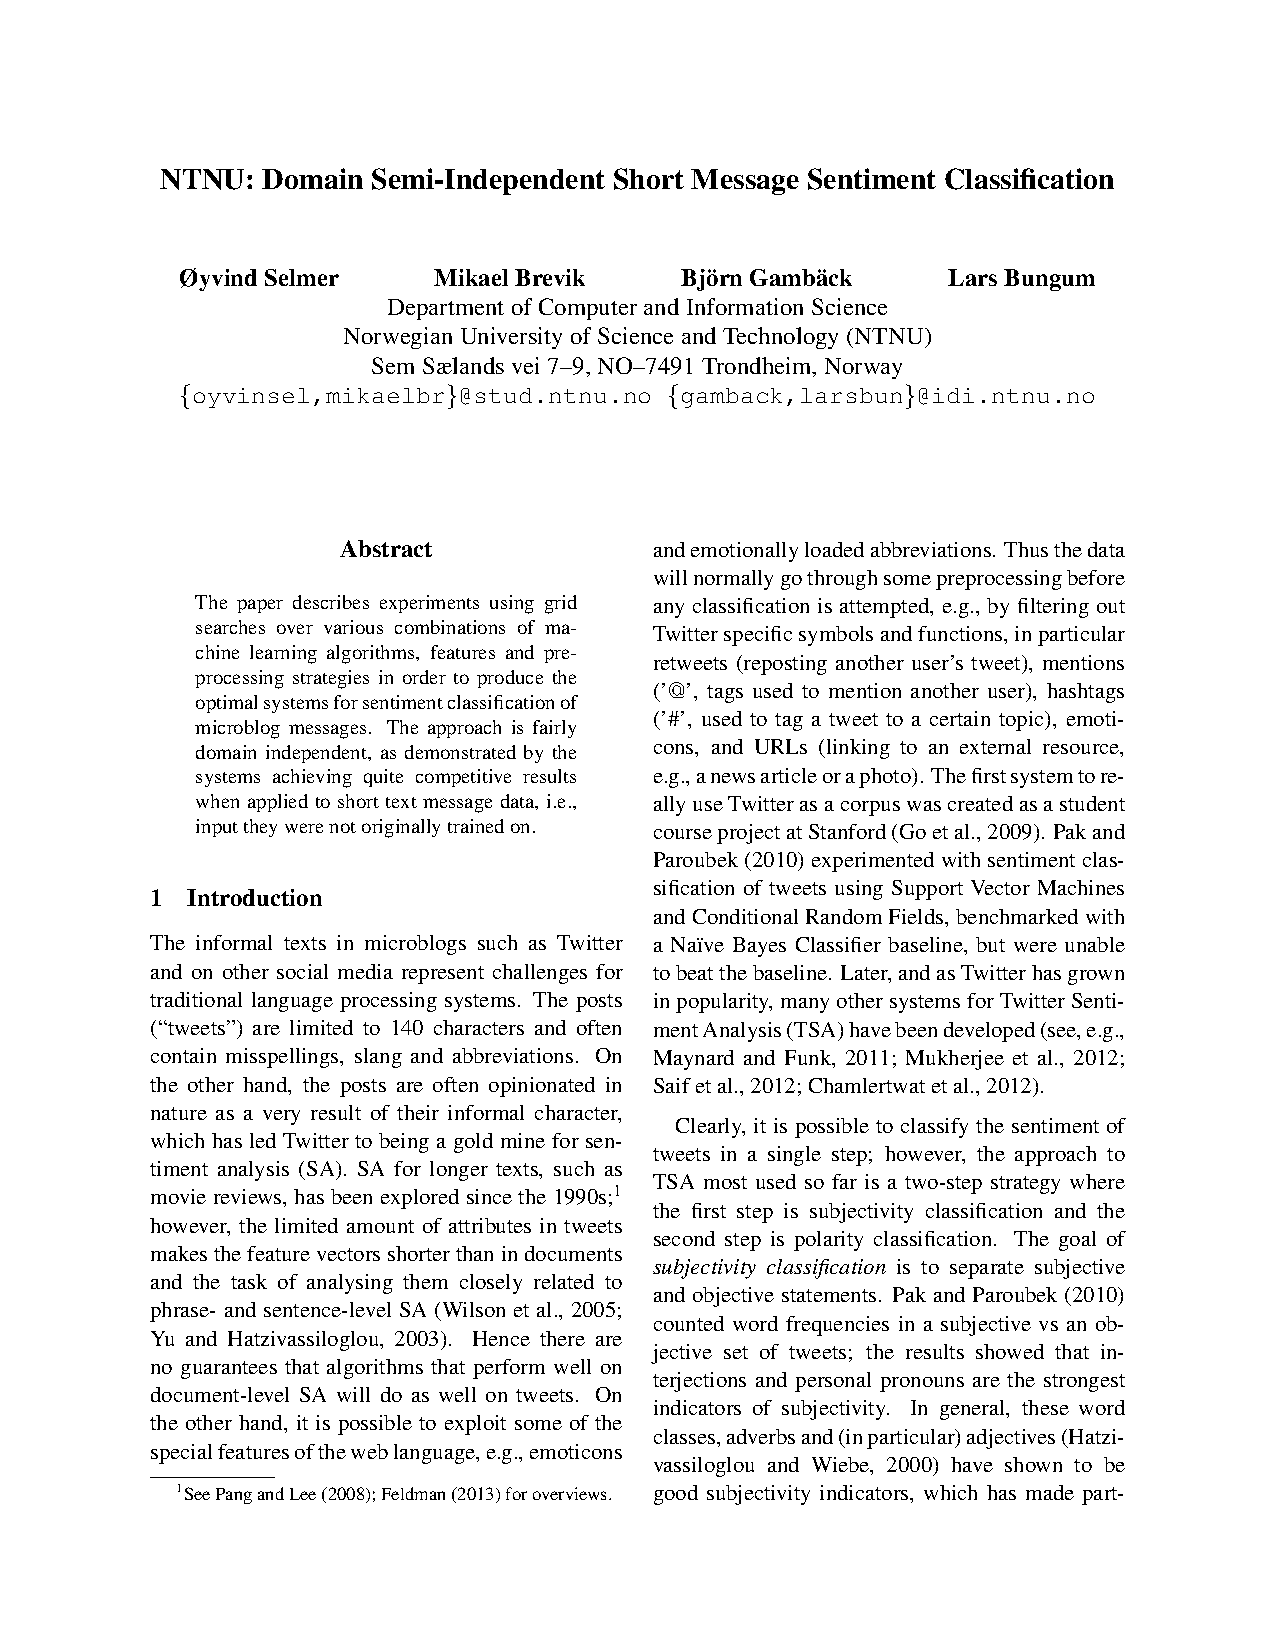
\includepdf[pages=-,pagecommand={\thispagestyle{empty}}]{selmerEA-v5.pdf}
\chapter{SemEval'13 Submitted Paper}
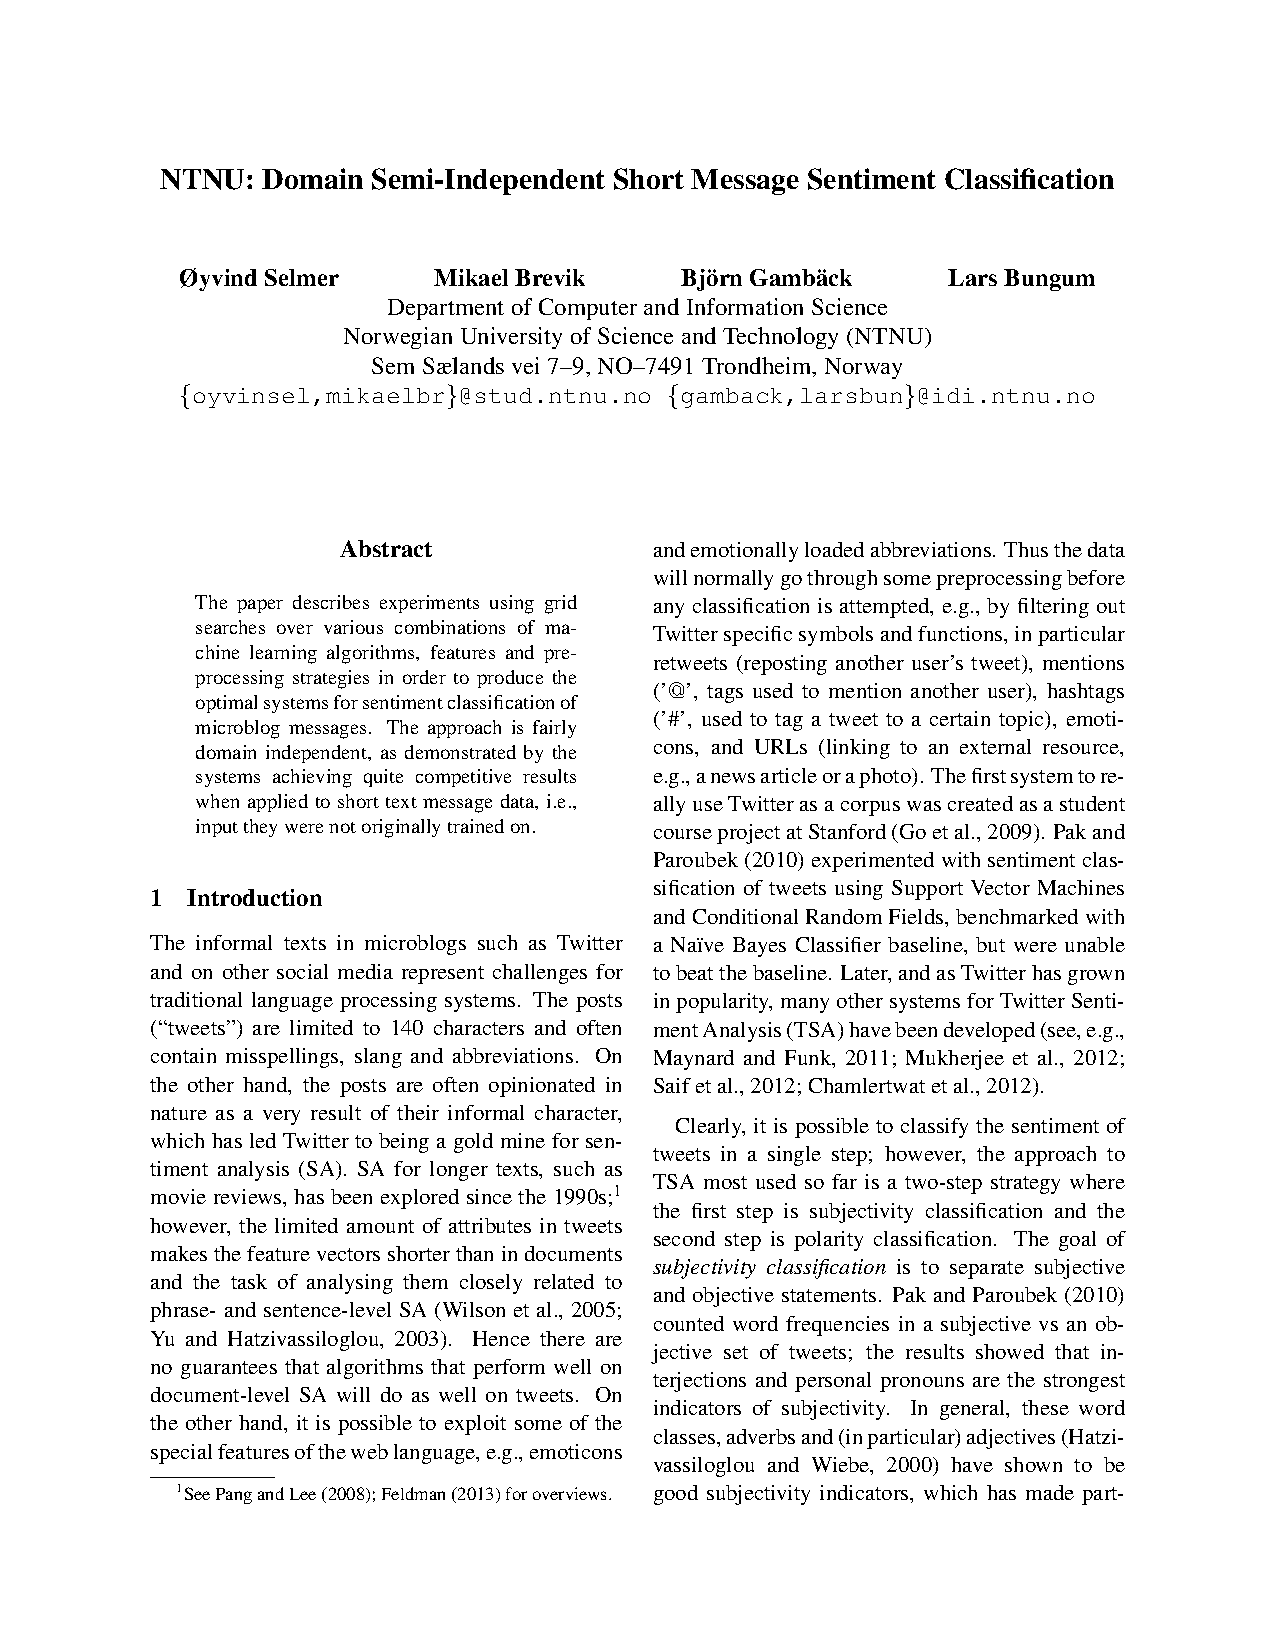
\includepdf[pages=-,pagecommand={\thispagestyle{empty}}]{selmerEA-v5.pdf}



\end{document}
